%%%%%%%%%%%%%%%%%%%%%%%%%%%%%%%%%%%%%%%%%%%%%%%%%%%%%%%%%%%%%%%%%%%%%%%%%%%%%%%%
%%%%%%%%%%%%%%%%%%%%%%%%%%%%%%%%%%%%%%%%%%%%%%%%%%%%%%%%%%%%%%%%%%%%%%%%%%%%%%%%
%%                                                                            %%
%% thesistemplate.tex version 4.01 (2023/09/21)                               %%
%% The LaTeX template file to be used with the aaltothesis.sty (version 4.00) %%
%% style file.                                                                %%
%% This package requires pdfx.sty v. 1.5.84 (2017/05/18) or newer.            %%
%%                                                                            %%
%% This is licensed under the terms of the MIT license below.                 %%
%%                                                                            %%
%% Written by Luis R.J. Costa.                                                %%
%% Currently developed at Teacher services, Learning Services of Aalto        %%
%% University by Luis R.J. Costa since May 2019.                              %%
%%                                                                            %%
%% Copyright 2017-2021 aaltothesis.cls by Luis R.J. Costa,                    %%
%% luis.costa@aalto.fi.                                                       %%
%% Copyright 2017-2018 Swedish translations in aaltothesis.cls by Elisabeth   %%
%% Nyberg and Henrik Wallén henrik.wallen@aalto.fi.                           %%
%% Finnish documentation in the template opinnatepohja.tex translated from    %%
%% the English template documentation.                                        %%
%% Copyright 2021 English template thesistemplate.tex by Luis R.J. Costa,     %%
%% Maurice Forget, Henrik Wallén.                                             %%
%% Copyright 2018-2022 Swedish template kandidatarbetsbotten.tex by Henrik    %%
%% Wallen.                                                                    %%
%%                                                                            %%
%% Permission is hereby granted, free of charge, to any person obtaining a    %%
%% copy of this software and associated documentation files (the "Software"), %%
%% to deal in the Software without restriction, including without limitation  %%
%% the rights to use, copy, modify, merge, publish, distribute, sublicense,   %%
%% and/or sell copies of the Software, and to permit persons to whom the      %%
%% Software is furnished to do so, subject to the following conditions:       %%
%% The above copyright notice and this permission notice shall be included in %%
%% all copies or substantial portions of the Software.                        %%
%% THE SOFTWARE IS PROVIDED "AS IS", WITHOUT WARRANTY OF ANY KIND, EXPRESS OR %%
%% IMPLIED, INCLUDING BUT NOT LIMITED TO THE WARRANTIES OF MERCHANTABILITY,   %%
%% FITNESS FOR A PARTICULAR PURPOSE AND NONINFRINGEMENT. IN NO EVENT SHALL    %%
%% THE AUTHORS OR COPYRIGHT HOLDERS BE LIABLE FOR ANY CLAIM, DAMAGES OR OTHER %%
%% LIABILITY, WHETHER IN AN ACTION OF CONTRACT, TORT OR OTHERWISE, ARISING    %%
%% FROM, OUT OF OR IN CONNECTION WITH THE SOFTWARE OR THE USE OR OTHER        %%
%% DEALINGS IN THE SOFTWARE.                                                  %%
%%                                                                            %%
%%                                                                            %%
%%%%%%%%%%%%%%%%%%%%%%%%%%%%%%%%%%%%%%%%%%%%%%%%%%%%%%%%%%%%%%%%%%%%%%%%%%%%%%%%
%%                                                                            %%
%%                                                                            %%
%% An example for writting your thesis using LaTeX                            %%
%% Original version and development work by Luis Costa, changes to the text   %% 
%% in the Finnish template by Perttu Puska.                                   %%
%% Support for Swedish added 15092014                                         %%
%% PDF/A-b support added on 15092017                                          %%
%% PDF/A-2 support added on 24042018                                          %%
%% Layout design and typesettin changed 15072021                              %%
%%                                                                            %%
%% This example consists of the files                                         %%
%%       thesistemplate.tex (version 4.00) (for text in English)              %%
%%       opinnaytepohja.tex (version 4.00) (for text in Finnish)              %%
%%       kandidatarbetsbotten.tex (version 1.10) (for text in Swedish)        %%
%%       aaltothesis.cls                                                      %%
%%       linediagram.pdf (graphics file)                                      %%
%%       curves.pdf      (graphics file)                                      %%
%%       ledspole.jpg    (graphics file)                                      %%
%%                                                                            %%
%%                                                                            %%
%% Typeset in Linux with                                                      %%
%% pdflatex: (recommended method)                                             %%
%%             $ pdflatex thesistemplate                                      %%
%%             $ pdflatex thesistemplate                                      %%
%%                                                                            %%
%%   The result is the file thesistemplate.pdf that is PDF/A compliant, if    %%
%%   you have chosen the proper \documenclass options (see comments below)    %%
%%   and your included graphics files have no problems.                       %%
%%                                                                            %%
%%                                                                            %%
%% Explanatory comments in this example begin with the characters %%, and     %%
%% changes that the user can make with the character %                        %%
%%                                                                            %%
%%%%%%%%%%%%%%%%%%%%%%%%%%%%%%%%%%%%%%%%%%%%%%%%%%%%%%%%%%%%%%%%%%%%%%%%%%%%%%%%
%%%%%%%%%%%%%%%%%%%%%%%%%%%%%%%%%%%%%%%%%%%%%%%%%%%%%%%%%%%%%%%%%%%%%%%%%%%%%%%%
%%
%% WHAT is PDF/A
%%
%% PDF/A is the ISO-standardized version of the pdf. The standard's goal is to
%% ensure that he file is reproducable even after a long time. PDF/A differs
%% from pdf in that it allows only those pdf features that support long-term
%% archiving of a file. For example, PDF/A requires that all used fonts are
%% embedded in the file, whereas a normal pdf can contain only a link to the
%% fonts in the system of the reader of the file. PDF/A also requires, among
%% other things, data on colour definition and the encryption used.
%% Currently three PDF/A standards exist:
%% PDF/A-1: based on PDF 1.4, standard ISO19005-1, published in 2005.
%%          Includes all the requirements essential for long-term archiving.
%% PDF/A-2: based on PDF 1.7, standard ISO19005-2, published in 2011.
%%          In addition to the above, it supports embedding of OpenType fonts,
%%          transparency in the colour definition and digital signatures.
%% PDF/A-3: based on PDF 1.7, standard ISO19005-3, published in 2012.
%%          Differs from the above only in that it allows embedding of files in
%%          any format (e.g., xml, csv, cad, spreadsheet or wordprocessing
%%          formats) into the pdf file.
%% PDF/A-4: based on PDF 2.0, standard ISO19005-4, published in November 2020.
%%
%% PDF/A-1 files are not necessarily PDF/A-2 -compatible and PDF/A-2 are not
%% necessarily PDF/A-1 -compatible.
%% Standards PDF/A-1, PDF/A-2 and PDF/A-3 have two levels:
%% b: (basic) requires that the visual appearance of the document is reliably
%%    reproduceable.
%% a (accessible) in addition to the b-level requirements, specifies how
%%   accessible the pdf file is to assistive software, say, for the physically
%%   impaired.
%% The PDF/A-4 standard does not have additional levels like in the earlier
%% standards.
%% For more details on PDF/A, see, e.g., 
%% https://www.loc.gov/preservation/digital/formats/fdd/fdd000318.shtml or
%% https://www.pdfa.org/resource/iso-19005-pdfa/
%%
%%
%% WHICH PDF/A standard should my thesis conform to?
%%
%% Either to the PDF/A-1b or the PDF/A-2b standard. If all the figures and
%% graphs used in thesis work do not require transparency features, use either
%% PDF/A-1b or PFDF/A-2b. If you have figures with transparency
%% characteristics, use the PDF/A-2b standard. However, drawing applications
%% often use the transparency parameter, setting it to zero, to specify opacity
%% and get the basic 2-D visualisation. As a result, validation of PDF/A-1b
%% will fail. Use PDF/A-2b if PDF/A-1b validation fails.
%% Do not use the PDF/A-3b standard for your thesis.
%% The font to be used are specified in this templatenand they should not be
%% changed. In addition to not adhering to Aalto's visual guidelines, you may
%% have difficulties in producing a PDF/A-compliant PDF.
%%
%%
%% Validate your PDF/A file at https://www.pdf-online.com/osa/validate.aspx
%%
%%
%% WHAT graphics format can I use to produce my PDF/A compliant file?
%%
%% When using pdflatex to compile your work, favour the use of pdf, but you can
%% use the jpg or png format especially for photographs. You will have PDF/A 
%% compliance problems with figures in pdf if the fonts are not embedded in the
%% pdf file.
%% If you choose to use latex to compile your work, the only acceptable file
%% format for your figure is eps. DO NOT use the ps format for your figures.

%% USE one of the following three \documentclass set-ups:
%% * the first when using pdflatex to directly typeset your document in the
%%   chosen pdf/a format for online publishing (centred page layout),
%% * the second for one-sided printing your thesis with the layout (wide left 
%%   margin), or
%% * the third for two-sided printing.
%%
\documentclass[english, 12pt, a4paper, sci, utf8, a-2b, online]{aaltothesis}
%\documentclass[english, 12pt, a4paper, elec, utf8, a-2b, print]{aaltothesis}
%\documentclass[english, 12pt, a4paper, elec, utf8, a-2b, print, twoside]{aaltothesis}

%% Use the following options in the \documentclass macro above:
%% your school: arts, biz, chem, elec, eng, sci
%% the character encoding scheme used by your editor: utf8, latin1
%% thesis language: english, finnish, swedish
%% make an archiveable PDF/A-1b or PDF/A-2b compliant file: a-1b, a-2b
%%                    (with pdflatex, a normal pdf containing metadata is
%%                     produced without the a-*b option)
%% typset for online document or print on paper: online, print
%%        online: typeset in symmetric layout and blue hypertext for online
%%                publishing
%%        print: typeset in a symmetric layout and black hypertext for printing
%%               on paper
%%          two-side printing: twoside (default is one-sided printing)
%%               typeset in a wide margin on the binding side of the page and
%%               black hypertext. Use with print only.
%%

%% Use one of these if you write in Finnish (or use the Finnish template
%% opinnaytepohja.tex)
%\documentclass[finnish, 12pt, a4paper, elec, utf8, a-1b, online]{aaltothesis}
%\documentclass[finnish, 12pt, a4paper, elec, utf8, a-1b, print]{aaltothesis}
%\documentclass[finnish, 12pt, a4paper, elec, utf8, a-1b, print, twoside]{aaltothesis}

%% Use one of these if you write in Swedish (or use the Swedish template
%% kandidatarbetsbotten.tex)
%\documentclass[swedish, 12pt, a4paper, elec, utf8, a-2b, online]{aaltothesis}
%\documentclass[swedish, 12pt, a4paper, elec, utf8, a-2b]{aaltothesis}
%\documentclass[swedish, 12pt, a4paper, elec, dvips, online]{aaltothesis}

%% FOR USERS OF AMS PACKAGES:
%% * newtxmath used in this template loads amsmath, so
%%   you needn't load it. If you want to use options in amsmath, load it here, 
%%   before \setupthesisfonts below to pass the options to amsmath.
%% * If you want to use amsthm, load it here before \setupthesisfonts to avoid
%%   a clash with newtxmath.
%% * If using amsmath with options and you want to use amsthm, load amsthms
%%   after amsmath, as described in the amsthm documentation.
%% * Don't use amsbsym or amsfonts. The symbols [and macros] there are defined in
%%   newtxmath and so clash if used.
%\usepackage[options]{amsmath}
%\usepackage{amsthm}

%% DO NOT MOVE OR REMOVE \setupthesisfonts
\setupthesisfonts

%% Add here the packges you need
%%
\usepackage{graphicx}
\usepackage{amsmath}
\newcommand{\Mod}[1]{\ (\mathrm{mod}\ #1)}%%
\usepackage{listings}
\usepackage{textcomp}

\lstalias[]{ES6}[ECMAScript2015]{JavaScript}

\lstdefinelanguage{JavaScript}{
  morekeywords=[1]{break, continue, delete, else, for, function, if, in,
    new, return, this, typeof, var, void, while, with},
  % Literals, primitive types, and reference types.
  morekeywords=[2]{false, null, true, boolean, number, undefined,
    Array, Boolean, Date, Math, Number, String, Object},
  % Built-ins.
  morekeywords=[3]{eval, parseInt, parseFloat, escape, unescape},
  sensitive,
  morecomment=[s]{/*}{*/},
  morecomment=[l]//,
  morecomment=[s]{/**}{*/}, % JavaDoc style comments
  morestring=[b]',
  morestring=[b]"
}[keywords, comments, strings]

\lstdefinelanguage[ECMAScript2015]{JavaScript}[]{JavaScript}{
  morekeywords=[1]{await, async, case, catch, class, const, default, do,
    enum, export, extends, finally, from, implements, import, instanceof,
    let, static, super, switch, throw, try},
  morestring=[b]` % Interpolation strings.
}

% Requires package: color.
\definecolor{mediumgray}{rgb}{0.3, 0.4, 0.4}
\definecolor{mediumblue}{rgb}{0.0, 0.0, 0.8}
\definecolor{forestgreen}{rgb}{0.13, 0.55, 0.13}
\definecolor{darkviolet}{rgb}{0.58, 0.0, 0.83}
\definecolor{royalblue}{rgb}{0.25, 0.41, 0.88}
\definecolor{crimson}{rgb}{0.86, 0.8, 0.24}

\lstdefinestyle{JSES6Base}{
  backgroundcolor=\color{white},
  basicstyle=\ttfamily,
  breakatwhitespace=false,
  breaklines=true,
  captionpos=b,
  columns=fullflexible,
  commentstyle=\color{mediumgray}\upshape,
  emph={},
  emphstyle=\color{crimson},
  extendedchars=true,  % requires inputenc
  fontadjust=true,
  frame=single,
  identifierstyle=\color{black},
  keepspaces=true,
  keywordstyle=\color{mediumblue},
  keywordstyle={[2]\color{darkviolet}},
  keywordstyle={[3]\color{royalblue}},
  numbers=left,
  numbersep=5pt,
  numberstyle=\tiny\color{black},
  rulecolor=\color{black},
  showlines=true,
  showspaces=false,
  showstringspaces=false,
  showtabs=false,
  stringstyle=\color{forestgreen},
  tabsize=2,
  title=\lstname,
  upquote=true  % requires textcomp
}

\lstdefinestyle{JavaScript}{
  language=JavaScript,
  style=JSES6Base
}
\lstdefinestyle{ES6}{
  language=ES6,
  style=JSES6Base
}



%% For tables that span multiple pages; used to split a paraphrasing example in
%% the appendix. If you don't need it, remove it.
\usepackage{longtable}

%% A package for generating Creative Commons copyright terms. If you don't use
%% the CC copyright terms, remove it, since otherwise undesired information may
%% be added to this document's metadata.
\usepackage[type={CC}, modifier={by-nc-sa}, version={4.0}]{doclicense}
%% Find below three examples for typesetting the CC license notice.

%\usepackage[square,numbers]{natbib}
\usepackage[natbib=true,firstinits=true,sorting=none]{biblatex}
\bibliography{references.bib}

% Used for inline code blocks
\usepackage{listings}

%\setcitestyle{numbers}
%% Edit to conform to your degree programme
%% Capitalise the words in the name of the degree programme: it's a name
\degreeprogram{Computer, Communication and Information Sciences}
%%

%% Your major
%%
\major{Security and Cloud computing}
%%

%% Choose one of the three below
%%
%\univdegree{BSc}
\univdegree{MSc}
%\univdegree{Lic}
%%

%% Your name (self explanatory...)
%%
\thesisauthor{Jonas Bäck}
%%

%% Your thesis title and possible subtitle comes here and possibly, again,
%% together with the Finnish or Swedish abstract. Do not hyphenate the title
%% (and subtitle), and avoid writing too long a title. Should LaTeX typeset a
%% long title (and/or subtitle) unsatisfactorily, you might have to force a
%% linebreak using the \\ control characters. In this case...
%% * Remember, the title should not be hyphenated!
%% * A possible 'and' in the title should not be the last word in the line; it
%%   begins the next line.
%% * Specify the title (and/or subtitle) again without the linebreak characters
%%   in the optional argument in box brackets. This is done because the title
%%   is part of the metadata in the pdf/a file, and the metadata cannot contain
%%   linebreaks.
%%
\thesistitle{Securing web clients utilizing OAuth 2.0}
%\thesistitle[Title of the thesis]{Title of\\ the thesis}
%%
%% Either remove or leave \thesissubtitle{} empty if you don't use it
%%
%\thesissubtitle{A possible subtitle}
%\thesissubtitle[Subtitle of the thesis]{Subtitle of\\ the thesis}
%\thesissubtitle{}

%%
\place{Espoo}
%%

%% The date for the bachelor's thesis is the day it is presented
%%
\date{3.6.2024}
%%

%% Thesis supervisor
%% Note the "\" character in the title after the period and before the space
%% and the following character string.
%% This is because the period is not the end of a sentence after which a
%% slightly longer space follows, but what is desired is a regular interword
%% space.
%%
\supervisor{Prof.\ Antti Ylä-Jääski}
%%

%% Advisor(s)---two at the most---of the thesis. Check with your supervisor how
%% many official advisors you can have.
%%
\advisor{M.Sc. Karri Lehtiranta}
%%

%% If you do your thesis work in a company of other institute, give the name of
%% the company or instution here. Otherwise, leave the macro empty, comment it
%% out, or remove it. This will remove this field from the abstract page.
%%
\collaborativepartner{twoday}
%%

%% Aaltologo: syntax:
%% \uselogo{?|!|''}
%% The logo language is set to be the same as the thesis language.
%%
%\uselogo{?}
%\uselogo{!}
\uselogo{''}
%%

%%%%%%%%%%%%%%%%%%               COPYRIGHT TEXT               %%%%%%%%%%%%%%%%%%
%%%%%%%%%%%%%%%%%%%%%%%%%%%%%%%%%%%%%%%%%%%%%%%%%%%%%%%%%%%%%%%%%%%%%%%%%%%%%%%%

%% Copyright of a work is with the creator/author of the work regardless of
%% whether the copyright mark is explicitly in the work or not. You may, if you
%% wish---we encourage you to do so---publish your work under a Creative
%% Commons license (see creativecommons.org), in which case the license text
%% must be visible in the work. Write here the copyright text you want using the
%% macro \copyrighttext, which writes the text into the metadata of the pdf file
%% as well.
%%
%% Syntax:
%% \copyrigthtext{metadata text}{text visible on the page}
%%
%% CHOOSE ONE OF THE COPYRIGHT NOTICE STYLES BELOW.
%% IF USING THE CC TERMS, CHOOSE THE LICENSE YOU WANT TO USE.
%% The different CC licenses are listed at 
%% https://creativecommons.org/about/cclicenses/.
%% If you use the icons from the dolicense.sty package, add the package above
%% (\usepackage{dolicense}).
%% IMPORTANT NOTE!! Manually write the CC text in the \copyrighttext metadata
%% text field.
%%
%% NOTE: In the macros below, the text written in the metadata must have a
%% \noexpand macro before the \copyright special character. When not in pdf/a
%% mode (i.e. a-1b or a-2b are not specified in \documentclass), two \noexpands
%% are required in the metadata text to correctly render the copyright mark in
%% the pdf metadata. In pdf/a mode one \noexpand suffices.
%%
%% EXAMPLE OF PLAIN COPYRIGHT TEXT
%% The macros \copyright and \year below must be separated by the \ character 
%% (space chacter) from the text that follows. The macros in the argument of the
%% \copyrighttext macro automatically insert the year and the author's name.
%% (Note! \ThesisAuthor is an internal macro of the aaltothesis.cls class file).
%%
%\copyrighttext{Copyright \noexpand\textcopyright\ \number\year\ \ThesisAuthor}
%{Copyright \textcopyright{} \number\year{} \ThesisAuthor}
%%
%% Of course, the same text could have simply been written as
%% \copyrighttext{Copyright \noexpand\copyright\ 2018 Eddie Engineer}
%% {Copyright \copyright{} 2022 Eddie Engineer}
%%
%% EXAMPLES OF CC LICENSE: different ways to display the same license
%% 1. A simple Creative Commons license text with a link to the copyright notice:
%\copyrighttext{\noexpand\textcopyright\ \number\year. This work is 
%	licensed under a CC BY-NC-SA 4.0 license.}{\textcopyright{} 
%	\number\year. This work is licensed under a 
%	\href{https://creativecommons.org/licenses/by-nc-nd/4.0/}{CC BY-NC-SA 4.0} 
%	license.}
%
%% To get the URL of the license of your choice, go to 
%% https://creativecommons.org/about/cclicenses/, click on the chosen license
%% you want to use, and copy-and-paste the URL in the macro \href above.
%%
%% 2. A short Creative Commons license text containing the respective CC icons
%% (requires the package dolicense.sty to be added in the preamble as done
%% above) and a link to the corresponding Creative Commons license webpage (see
%% the dolicense package documentation for other license icons):
%\copyrighttext{\noexpand\textcopyright\ \number\year. This work is licensed
%	under a CC BY-NC-SA 4.0 license.}{
%	\parbox{95mm}{\noindent\textcopyright\ \number\year. \doclicenseText} 
%	\hspace{1em}\parbox{35mm}{\doclicenseImage}
%}
%%
%% 3. An expanded Creative Commons license text containing the respective CC
%% icons text and as generated by the dolicense.sty package (the license is set
%% via package options in \usepackage[options]{dolicense} above; see the
%% dolicense package documentation for other license texts and icons):
\copyrighttext{\noexpand\textcopyright\ \number\year. This work is 
	licensed under a Creative Commons "Attribution-NonCommercial-ShareAlike 4.0 
	International" (BY-NC-SA 4.0) license.}{\noindent\textcopyright\ \number
	\year \ \doclicenseThis}
%%%%%%%%%%%%%%%%%%%%%%%%%%%%%%%%%%%%%%%%%%%%%%%%%%%%%%%%%%%%%%%%%%%%%%%%%%%%%%%%


%% The English abstract:
%% All the details (name, title, etc.) on the abstract page appear as specified
%% above.
%% Thesis keywords:
%% Note! The keywords are separated using the \spc macro
%%
\keywords{OAuth 2.0, single sign-on, web development, security, authentication, authorization}
%%

%% The abstract text. This text in one paragraph is included in the metadata of
%% the pdf file as well as the abstract page. To have paragraphs in your
%% abstract rewrite it in the abstarct environment as described below.
%%

\thesisabstract{%
The abstract is a short description of the essential contents of the thesis
usually in one paragraph: what was studied and how and what were the main
findings. For a Finnish thesis, the abstract should be written in both Finnish
and English; for a Swedish thesis, in Swedish and English. The abstracts for
English theses written by Finnish or Swedish speakers should be written in
English and either in Finnish or in Swedish, depending on the student’s language
of basic education. Students educated in languages other than Finnish or Swedish
write the abstract only in English. Students may include a second or third
abstract in their native language, if they wish. 
The abstract text of this thesis is written on the readable abstract page as
well as into the pdf file's metadata via the thesisabstract macro (see the 
comment in the TeX file). Write here the text that goes into the metadata. The 
metadata cannot contain special characters, linebreak or paragraph break 
characters, so these must not be used here. If your abstract does not contain 
special characters and it does not require paragraphs, you may take advantage of
the abstracttext macro (see the comment in the TeX file below). Otherwise, the 
metadata abstract text must be identical to the text on the abstract page.
}


%% You can prevent LaTeX from writing into the xmpdata file (it contains all the 
%% metadata to be written into the pdf file) by setting the writexmpdata switch
%% to 'false'. This allows you to write the metadata in the correct format
%% directly into the file thesistemplate.xmpdata.
%\setboolean{writexmpdatafile}{false}


%% All that is printed on paper starts here
%%

\begin{document}

%% Create the coverpage
%%
\makecoverpage

%% Typeset the copyright text.
%% If you wish, you may leave out the copyright text from the human-readable
%% page of the pdf file. This may seem like a attractive idea for the printed
%% document especially if "Copyright (c) yyyy Eddie Engineer" is the only text
%% on the page. However, the recommendation is to print this copyright text.
%%
\thispagestyle{empty}%
%  \vspace*{-25mm}%
%  \noindent%
%  \mbox{\@@ltoabslogo}\par% this is the logo
%  \vspace*{25mm}%
  \noindent%
  Copyright \textcopyright \ 2024   Jonas Bäck
  \clearpage

%\makecopyrightpage

\clearpage
%% Note that when writing your thesis in English, place the English abstract
%% first followed by the possible Finnish or Swedish abstract.

%% Abstract text
%% All the details (name, title, etc.) on the abstract page appear as specified
%% above. Add your abstarct text with paragraphs here to have paragraphs in the
%% visible abstract page. Nonetheless, write the abstarct text without
%% paragraphs in the macro \thesismacro so that it is added to the metadata as
%% well.
%%

\begin{abstractpage}[english]
The OAuth 2.0 specification is widely used to authorize applications to use resources belonging to third parties and to enable single sign-on across multiple applications.
While the technology is widely used, the lax nature of the specification leaves plenty of different options for developers looking to implement the specification, enabling different OAuth systems to have very different security characteristics.
As third-party OAuth authorization servers are often utilized by developers that might have limited knowledge of the technology and might thus be unaware of the security implications of their choices, this thesis aims to present known vulnerabilities in OAuth systems, and demonstrates simple steps that should be taken to securely implement the specification.

This thesis presents a number of vulnerabilities of varying severity that are common in real-world systems utilizing OAuth.
These vulnerabilities are often caused by incorrect implementation of OAuth clients and authorization servers, but the lax nature of the specification allowing the creation of insecure applications if only the bare minimum of the specification is implemented is an equally common source for vulnerabilities.
Through a practical client implementation utilizing third-party authorization servers, this thesis shows that a number of simple steps can be taken to mitigate many of the described vulnerabilities, often at a minimal development and performance cost and without a significant increase in complexity.
It is however not always obvious if the most secure option is the optimal choice for a specific system, such as when deciding if and how to persist user sessions, as a more secure option might lead to a deterioration in user experience.
To help developers adapt the OAuth specification to their specific application according to their security requirements, this thesis presents the impact of different design choices and shows why taking extra precautions is often worth the effort.
\end{abstractpage}

%% The text in the \thesisabstract macro is stored in the macro \abstractext, so
%% you can use the text metadata abstract directly as follows:
%%
%\begin{abstractpage}[english]
%	\abstracttext{}
%\end{abstractpage}

%% Force a new page so that the possible Finnish or Swedish abstract does not
%% begin on the same page
%%

%% Force new page so that the Swedish abstract starts from a new page
\newpage

%% Swedish abstract. Delete it if you don't need it. 
%% 
%% Respecify those fields that differ from the earlier specification or simply
%% respecify all fields.
\thesistitle{Säkrande av webbklienter som utnyttjar OAuth 2.0}
\supervisor{Prof.\ Antti Ylä-Jääski}
\advisor{D.I. Karri Lehtiranta}
\degreeprogram{Computer, Communication and Information Sciences}
%\collaborativepartner{twoday}
%\date{21.9.2023}
%% Abstract keywords
\keywords{OAuth 2.0, webbutveckling, säkerhet, autentisering,
auktorisering}
%% Abstract text
\begin{abstractpage}[swedish]
OAuth 2.0-specifikationen används ofta för att auktorisera applikationer att använda resurser som tillhör tredje parter och för att möjliggöra att användare autentiseras med samma konto i flera applikationer.
Även om teknologin används i stor utsträckning ställer specifikationen få krav på utvecklare, vilket möjliggör många olika alternativ då teknologin implementeras.
Denna brist på strikta krav gör det möjligt för varierande applikationer att utnyttja teknologin, men det leder också till att olika OAuth-system kan ha väldigt olika säkerhetsegenskaper.
OAuth auktoriseringsservrar som upprätthålls av tredje parter utnyttjas ofta av utvecklare för autentisering, vilket leder till att utvecklare slipper implementera komplicerade inloggningssystem för att autentisera sina användare.
Då utvecklare kan utnyttja OAuth servrar och implementera OAuth klienter utan djupare kunskap om teknologin är det lätt hänt att beslut om hur systemet ska implementeras tas utan att ta säkerhetskonsekvenserna i beaktande.
Målet med denna avhandling är att presentera kända sårbarheter i OAuth-system och beskriva enkla steg som bör tas för att implementera specifikationen på ett säkert sätt.

I denna avhandling presenteras ett antal sårbarheter av varierande allvarlighetsgrad som är vanliga i system som använder OAuth.
Dessa sårbarheter orsakas ofta av felaktig implementering av OAuth-klienter och auktoriseringsservrar, men bristen på strikta krav i specifikationen som gör det möjligt att skapa osäkra applikationer utan att göra explicita fel är en lika vanlig källa till sårbarheter.
Genom en praktisk implementation av en OAuth-klient som utnyttjar tredje parters auktoriseringsservrar visar denna avhandling att ett antal enkla steg kan tas för att minska många av de beskrivna sårbarheterna, ofta till en minimal kostnad och utan en betydande ökning av komplexitet.
Det är dock inte alltid uppenbart om det säkraste alternativet är det optimala valet för ett visst system, exempelvis då man ska besluta om och hur användarsessioner ska bevaras, eftersom ett säkrare alternativ kan leda till en försämrad användarupplevelse.
För att hjälpa utvecklare att anpassa OAuth-specifikationen till sin specifika applikation i enlighet med sina säkerhetskrav presenterar avhandlingen effekterna av olika beslut då OAuth-system implementeras och visar varför det ofta är värt besväret att vidta extra åtgärder för att göra system tillräckligt säkra.
\end{abstractpage}


\dothesispagenumbering{}

%% Preface
%%
%% This section is optional. Remove it if you do not want a preface.
%\mysection{Preface}
%\mysection{Esipuhe}
%I want to thank Professor Pirjo Professor and my instructors Dr Alan Advisor and
%Ms Elsa Expert for their guidance.

%I also want to thank my partner for keeping me sane and alive.

%\vspace{5cm}
%Otaniemi, 9 February 2023\\

%\vspace{5mm}
%{\hfill Eddie E.\ Engineer \hspace{1cm}}

%% Force a new page after the preface
%%
\newpage


%% Table of contents. 
%%
\thesistableofcontents


%% Symbols and abbreviations
\mysection{Abbreviations}

\begin{tabular}{ll}
HTTP       & Hypertext transfer protocol \\
HTTPS      & Hypertext transfer protocol secure \\
TLS        & Transport layer security \\
OIDC       & OpenID connect \\
SSO        & Single sign-on \\
HTML       & HyperText markup language \\
CSS        & Cascading style sheets \\
SEO        & Search engine optimization \\
RIA        & Rich internet application \\
SPA        & Single-page application \\
JSON       & JavaScript object notation \\
Ajax       & Asynchronous JavaScript and XML \\
API        & Application programming interface \\
IdP        & Identity provider \\
MFA        & Multi-factor authentication \\
URI        & Uniform resource identifier \\
XSS        & Cross-site scripting \\
PKCE       & Proof key for code exchange \\
CSRF       & Cross site request forgery 

\end{tabular}


%% \clearpage is similar to \newpage, but it also flushes the floats (figures
%% and tables).
%%
\cleardoublepage


%% Text body begins. Note that since the text body is mostly in Finnish the
%% majority of comments are also in Finnish after this point. There is no point
%% in explaining Finnish-language specific thesis conventions in English.
%% This text will be translated to English soon.
%%

\section{Introduction}
\label{sec:intro}

%% Leave page number of the first page empty
%% 
\thispagestyle{empty}

In recent years, single sign-on (SSO) systems have become common, allowing users to authenticate using one centralized account.
SSO systems can help secure user authentication by mitigating password fatigue and password reuse \citep{dhamija_seven_2008}, in addition to creating a more convenient user experience by removing the need for the user to authenticate on each web application separately.
Additionally, SSO systems remove the need for each web application to implement their own authentication system, allowing a smaller number of centralized actors with the required resources to implement the systems securely.

OAuth 2.0 is an open standard that is commonly used by SSO systems that allow users to share information about their account with third parties, allowing the third party to use the SSO system to authenticate their users \citep{fett_comprehensive_2016}.
The OAuth specification defines how authorization servers function and how they should be interacted with.
The specification does not however define how the client interacting with the authorization server should be implemented, leaving room for potential developer mistakes and unintended vulnerabilities.
The popularity of OAuth makes it a tempting attack vector, further increasing the chance that any vulnerabilities in the client implementation will be exploited.

\subsection{Problem statement}

The OAuth 2.0 specification is widely used today.
The specification is however not very strict, leaving plenty of room for developers to implement the system as they like.
While this does enable a wide variety of systems to utilize OAuth, it means that two different systems implementing the same specification might not be as secure.
As the specification is quite well studied, a number of common vulnerabilities are known, with well defined defenses.
Some of these defenses are described as recommendations in the OAuth specification, while other solutions might only be described in third-party sources.

As SSO-systems are typically used by developers to lower the required amount of logic needed to implement authentication, it is not only essential that it is easy to implement an OAuth client, but that it is easy to implement a secure client.
There are a number of different options that are available when implementing an OAuth client, and it is important to consider the security implications of these decisions.
While the specification might allow certain implementation options, understanding the negative effect on the system's security should help developers consider other options, leading to a more secure system.
Multiple widely used open-source OAuth clients  exist, but their implementations can vary significantly and the motivation behind their choices is not always well defined.
Additionally, the OAuth clients are often implemented by and for a specific identity provider, forcing developers to implement their own client or combining multiple clients if they want to support multiple providers.
Different client platforms also come with specific security considerations; this thesis will however focus on JavaScript-based web clients.

This thesis aims to achieve the following objectives:
\begin{enumerate}
    \item \textbf{Identify common vulnerabilities in OAuth clients} \\
    To be able to securely implement OAuth-based authentication, it is essential to understand common vulnerabilities, both in OAuth clients and authorization servers.
    \item \textbf{Demonstrate a secure client implementation} \\
    The second objective is to implement a secure OAuth web-client using JavaScript and to demonstrate how the previously shown vulnerabilities are mitigated.
\end{enumerate}

\subsection{Structure of the thesis}

Chapter 2 offers an overview of relevant technologies when inspecting the security of OAuth web clients, 
providing information on how web traffic is secured and how web applications are typically structured.
Chapter 3 gives an overview of the OAuth 2.0 specification and describes how it can be used to authenticate users.
Chapter 4 investigates common vulnerabilities in OAuth systems.
Chapter 5 presents a JavaScript-based OAuth client which attempts to mitigate the vulnerabilities found in chapter 4.
Chapter 6 discusses the implementation of chapter 5 and how it takes the vulnerabilities of chapter 4 into account. The chapter also lists observations from utilizing a third-party authorization server, focusing on the quality of documentation as well as on how the authorization servers have been implemented.
Chapter 7 summarizes the key results of the study.


%% In a thesis, every section/chapter starts a new page, hence the \clearpage
\clearpage

\section{Background}
\label{sec:background}

This section gives an overview of the areas that are required to evaluate the security of an OAuth system.
Since the OAuth specification deals with transmitting sensitive data over the internet, the first section describes how network communication can be secured, with details on public key encryption and Transport Layer Security.
The second section describes the structure of web applications, considering the different implementation options that are available today as well as their security considerations.
To be able to evaluate different methods for storing OAuth user identifiers, the third section details the different options that are available for storing data in web clients.
The fourth section describes different methods that can be used to authenticate HTTP communication.
The fifth section describes cross-site request forgery attacks, which is a common attack type that is especially relevant in the context of OAuth.


\subsection{Securing network traffic}
The complex and distributed nature of the internet causes it to be inherently insecure. A network request may travel through switches located in a number of countries and operated by various actors, and the route might even change between requests as the network topology and load changes. As such, we have to assume that some link along the chain is listening to the traffic we send. In the context of web traffic, this lack of trust causes issues, as users want to be able to send potentially sensitive information with the knowledge that no external actor will be able to read or modify the data.

\subsubsection{Public key encryption}
To mitigate the risk of malicious parties being able to listen in on network communication, public-key encryption can be used.
Public key cryptography relies on a public-private key pair, where the public key is used to encrypt data and the private key is used to decrypt data.
A network actor can generate the key pair and send the public key to the other endpoint.
Since the public key can only be used to encrypt data, an attacker will not gain any valuable information if they are able to intercept the public key.
With the public key, the other endpoint can encrypt the data before sending it over a network.
Since the data can only be decrypted by the corresponding private key, a network attacker which successfully intercepts the communication is unable to read the original data \citep{hellman_overview_1978}.

Diffie-Hellman key exchange is one method to exchange keys for public key cryptography \citep{diffie_new_1976}  \citep{gillmor_negotiated_2016}.
\begin{enumerate}
    \item The Diffie-Hellman key exchange begins by two parties, Alice and Bob, agreeing on two publicly shared values, $p$, and $g$, where $p$ is a prime and $g$ is a primitive root modulo $p$.
    \item Alice chooses a secret integer $a$ and sends $A = g^a \mod p$ to Bob.
    \item Bob chooses a secret value $b$ and sends $B = g^b \mod p$ to Alice.
    \item Alice computes $s = B^a \mod p$
    \item Bob computes $s = A^b \mod p$
\end{enumerate}

Alice and Bob now share the secret $s$, since \[A^b \mod p = g^{ab} \mod p = g^{ba} \mod p = B^a \mod p\]
The secret share is considered secure, as finding $a$ and $b$ given $g^{ab} \mod p = g^{ba} \mod p$ takes a long time to compute with our current algorithms.

If Diffie-Hellman key exchange is used, an attacker can store large amounts of network traffic, with the hope of the secret key leaking in the future, thus allowing the attacker to decrypt all previous communication.
Additionally, in traditional public-key cryptography, the keys between two parties can stay constant for long amounts of time, allowing an attacker to decrypt all previous traffic at once if the secret is leaked in the future.
To protect against such attacks, short lived keys, commonly referred to as ephemeral keys, can be used, such as in the SAKE protocol \citep{jarecki_symmetric-key_2020}.
The SAKE protocol solves the issue of a future key leak being able to decrypt previous communication by continuously updating the secret key, making it impossible to derive an older secret key from a newer one.
Ensuring that an encryption scheme is resistant to keys being leaked at a later point is known as perfect forward secrecy.

\subsubsection{Transport Layer Security}
Today, the Transport Layer Security (TLS) protocol is used to prevent eavesdropping, tampering and forging messages in client-server communication. The latest version of the specification is TLS 1.3, which among other things removes insecure ciphers, allows for fewer round trips in the handshake and forces clients and servers to use ephemeral key exchange methods, ensuring perfect forward secrecy \citep{dowling_cryptographic_2015}. 

TLS provides a secure channel which provides authentication, confidentiality and integrity, even if an attacker has complete control of the network. The server is always authenticated, while the client can be optionally authenticated. The confidentiality of the transmitted data is ensured by encryption, only allowing the server and client to decrypt the contents. TLS 1.3 additionally ensures forward secrecy, effectively preventing attacks that store large amounts of encrypted data with the hope of decrypting it at a later point when keys are compromised. The lengths of the data and the identities of the client and server are however not hidden. Integrity is ensured by detecting any external modifications to the sent data.

The full TLS 1.3 handshake, described in figure \ref{tls}, functions as follows \citep{rescorla_transport_2018}:

\begin{figure}[b]
	\centering
	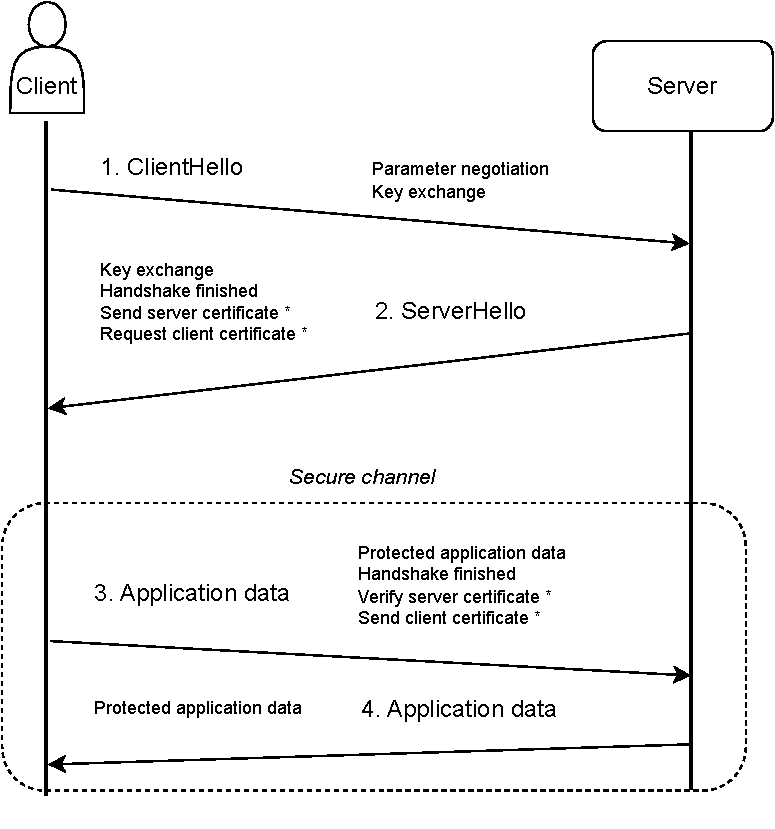
\includegraphics[height=120mm]{assets/tls_1.3_handshake.drawio.pdf}
	\caption{Full TLS 1.3 handshake. Optional content marked with *.}
	\label{tls}
\end{figure}

\begin{enumerate}
    \item The \textit{ClientHello} message is used for negotiating parameters and exchanging keys. The configurable parameters are TLS versions, groups, cipher suites and certificate authorities. The key exchange is initiated by sending the client's Diffie-Hellman key share. The client can request a server certificate, further ensuring that no impersonation attack can take place.
    \item \textit{ServerHello}: The server selects a cipher and TLS version based on the lists sent by the client and confirms that the handshake is finished. The server can suggest new parameters if it does not support any of the parameters sent by the client. The server also sends its own Diffie-Hellman key share and a server certificate, if one was requested. If client authentication is used, the server will request a client certificate. If a pre-shared key is used, the server can send application data in this message, allowing for data transfer without any additional round trips.
    \item A secure channel is established, allowing the client to send application data encrypted with the previously shared key. The client confirms that the handshake has been completed and sends a certificate if one was requested.
    \item The server can now use the secure channel to send encrypted application data.
\end{enumerate}

\clearpage
\subsection{Structure of web applications}
\label{sec:background-structure}

Web pages can be characterized by clients fetching web pages from servers and displaying the pages in web browsers. The basic building blocks for a web page are HyperText Markup Language (HTML) elements, which describe the structure and content of the page. The layout and style of web pages can be modified by using Cascading Style Sheets (CSS). The addition of JavaScript makes it possible for the browser to execute arbitrary code, greatly improving the options for interactive pages. 
Since its inception in the 80's, the web has evolved and matured. From static, read-only pages utilizing HTML to pages allowing users to write and participate in the web during the turn of the millennium, made possible in part by the adoption of JavaScript. The evolution continued to allow users to execute programs that we commonly refer to as web applications today \citep{jacksi_development_2019}. 


\subsubsection{Static web pages}
A traditional, static web page is stored in its entirety on the server and is served to users on request. 
Such pages typically require only HTML and CSS to function.
As the client side barely includes any logic, the focus is on the server, which stores and serves data and handles all business logic.
Navigation and interaction with the page is done using clickable links that direct the user to other pages.
Figure \ref{static} describes a user visiting a web page \textit{example.com}, clicking a link to visit \textit{example.com/apply} and finally submitting a form to \textit{example.com/apply}.
Keeping the content strictly separated in pages and serving the complete page as-is to clients provides a number of benefits \citep{camden_why_nodate}:

\begin{itemize}
    \item The amount of data transferred when visiting a site is low, as only the content that is immediately shown to the user has to be sent. This speeds up load times for the end user, reduces data usage and typically leads to a lower delay before content is visible in the browser.
    \item Static websites are typically easier to traverse programmatically than dynamic sites. This makes it easier for web crawlers to index the site, such as those used by search engines, making search engine optimization (SEO) trivial. Additionally, static sites are typically more accessible as they can be parsed more easily by screen readers and similar software \citep{okoye_accessibility_2014}.
    \item As the use of JavaScript allows websites to execute near arbitrary code in browsers, users can choose to disable JavaScript altogether. This will cause most dynamic sites to stop working, while static websites can function without using JavaScript. This removes the option for potential attackers to execute harmful code on the user's machine and often limits the tracking capabilities of websites. 
\end{itemize}

There are, however, reasons why strictly static sites are rare today, compared to the early days of the web when they were the standard \citep{nath_web_2014}:

\begin{itemize}
    \item Static websites are slow and clunky to use, as any interaction with the site requires the client to fetch a new page, or reload the current page from the server.
    \item Static websites only support client-initiated requests, making it impossible for the server to implement event-driven patterns, such as sending notifications to the client.
    \item Continually updating pages is not possible, as doing so would require server-initiated communication. The problem could be solved by the client periodically requesting the latest data, but this is not possible in strictly static sites as it requires JavaScript to implement.
\end{itemize}

\begin{figure}[b]
	\centering
	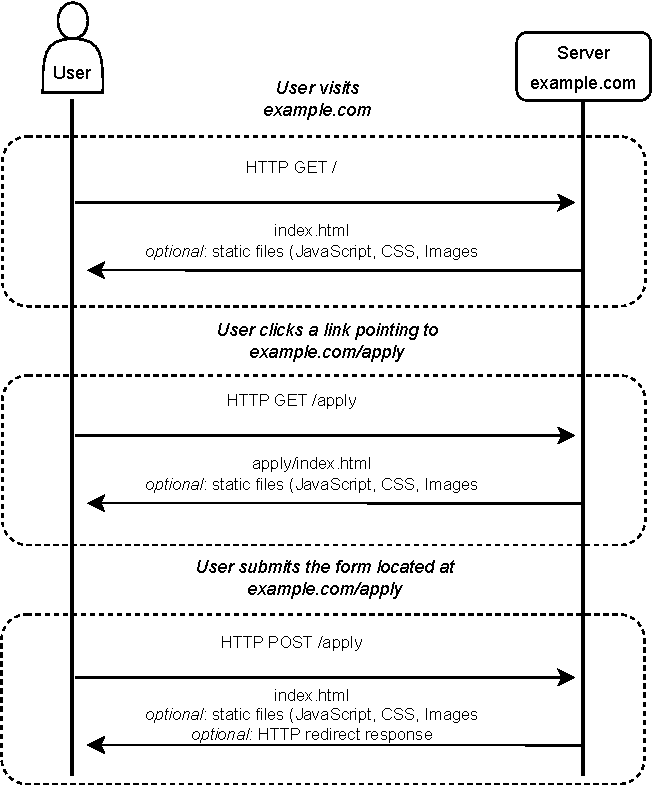
\includegraphics[height=120mm]{assets/http_request.drawio.pdf}
	\caption{Network traffic for a user interacting with a static web site.}
	\label{static}
\end{figure}

\subsubsection{Rich internet applications}

To allow for client-side scripting and alleviate some of the issues with strictly static sites, JavaScript was introduced in the mid 90's. While this allowed developers to create dynamic user interfaces, web apps as we know them today did not become popular until the introduction of third-party tools, such as Adobe Flash and Java in web apps. These technologies allowed for the development of rich internet applications (RIAs) that delegated some logic and data storage to the client, while using separate HTML pages for different pages \citep{fraternali_rich_2010}.
While these tools allowed for the creation of interactive web apps, end users had to install the tools separately if they wanted to utilize them. In addition to being a hassle for end users, these plugins introduced additional security vulnerabilities. At the time of writing, 1084 common vulnerabilities and exposures (CVEs) have been reported for Adobe Flash \citep{noauthor_adobe_nodate}.

Some way to create interactive web apps using only HTML, CSS and JavaScript was needed. The adoption of Asynchronous JavaScript and XML (Ajax) around 2005 saw web development move towards JavaScript-based applications that are common today. 
The asynchronous nature of Ajax allowed for completing network requests in the background without blocking user input and updating relevant parts of the interface when the request completed. 
JavaScript-based abstractions built on top of Ajax made development easier, such as jQuery \citep{openjsforg_jquery_nodate}, released in 2006, and the fetch() function \citep{noauthor_fetch_2023}, released in 2015. 

\subsubsection{Single-page applications}

Logic can further be delegated to the client, allowing for single-page applications (SPAs), that contain all the web pages for an application in one HTML page
\citep{fink_introducing_2014}. 
While the name might imply that SPAs only have one page, they can have any number of pages visible from the end users point of view, with the term \textit{single page} referring to the number of HTML pages.
In contrast to static web applications and RIAs, SPAs use client side logic instead of full HTTP requests to handle navigation and user input.
This often leads to improved responsiveness for users and makes dealing with client-side data and state easier, at the cost of a longer initial load time due to the larger size of the page.
The backend typically consists of an application programming interface (API), which is designed for machine communication with responses that might not be easily human-readable.
The backend and frontend often utilize JavaScript Object Notation (JSON) data to communicate.

Figure \ref{spa} shows the network traffic between a user and a web server for a simple SPA.
When comparing the traffic with the static page traffic in figure 2, the static page always returns a complete HTML page and redirects the user accordingly, while the SPA only fetches one HTML page on the initial page load.
The requests for the user navigating to \textit{/apply} and the user submitting a form can be identical for both the static page and the SPA.
The response from the backend is however different, with the static application returning a complete page and the SPA returning data in any suitable format, typically JSON.

\begin{figure}[b]
	\centering
	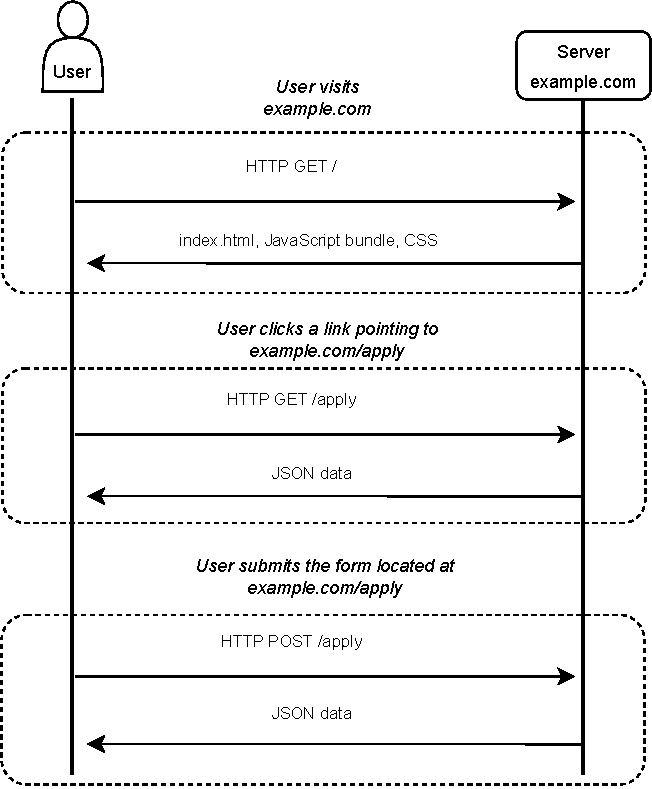
\includegraphics[height=120mm]{assets/spa_http_request.drawio.pdf}
	\caption{Network traffic for a user interacting with a Single Page Application.}
	\label{spa}
\end{figure}

While the network traffic of the SPA and static web page might seem very similar at first, there are many practical differences \citep{fink_introducing_2014}.
As SPAs implement navigation in the client, user navigation could be achieved without any network traffic, completely relying on the content of the first page load.
In practice some network traffic is often useful when navigating a SPA. 
Dynamic information can be fetched on navigation, periodically by the client or on-demand by the server, as data fetched on initial page load could easily become stale.
Pre-rendered HTML and static content such as images can also be fetched on navigation, lowering the size of the initial HTML page.
With SPAs, developers are given greater freedom in implementation, having the option to develop web applications very similarly to native applications, while not requiring end users to install anything on their machines.
While moving much of the logic to the client can make applications more responsive, moving logic from an opaque server to a transparent client application requires developers to pay attention to which parts they could move to the client.
In general, developers should assume that all data and application logic that is located in the client can be freely accessed and modified by potential attackers.


\subsection{Client-side storage}
\label{sec:background-storage}

In web applications that execute code on the client, storing data in the client browser is often required.
The use of JavaScript allows developers to store data in variables, making it possible to keep track of application state and to create more complex programs.
It is often useful to persist data over different sessions, and as JavaScript variables are cleared when refreshing the page, other methods for storing data are needed.
A common use case for persistent storage methods is keeping track of users by storing a session token in the client browser, allowing authenticated users to navigate a web page without having to authenticate every time they visit a new page.

\subsubsection{Cookies}
\label{sec:background-storage-cookies}
Cookies have long been used to allow servers to store state at HTTP user agents, such as web browsers, over the HTTP protocol, which itself is mostly stateless.
Cookies function by passing data in HTTP headers.
By using the Set-Cookie field, servers can pass name/value pairs and related metadata to user agents.
In later requests, the user agent can set a previously stored value in the Cookie field, allowing the server to identify the client or to keep track of user preferences.
Cookies are not always suitable for keeping track of user state or identifiers.
Using cookies, a server cannot differentiate between different sessions for one user.
As an example, if a user had two separate windows open at the same time and was trying to purchase two different items, the session would leak between the two windows \citep{noauthor_html_nodate}.
Cookies are also limited by their max size, which is 4096 bytes.

When setting cookies, the server can define the scope of the cookie, which can include the domain and path of the cookie, as well as if it should be allowed to be used in HTTP requests that do not use TLS
\citep{barth_rfc6265_2011}.
The use of scope for cookies is essential if it contains confidential information such as session identifiers.
If a domain is not defined for the cookie, the value could be read by any visited website, significantly increasing the chance for session hijacking.
Similarly, if the cookie is allowed to be used without TLS, any network attacker would be able to read the transmitted data.
To limit many vulnerabilities, such as cross-site scripting (XSS) attacks, the \textit{HttpOnly} flag can be set for cookies that are used as session identifiers.
The flag blocks access to the cookie from JavaScript executed in the client, only allowing it to be sent as part of a request in the Cookie header.

To further protect against cross-site attacks, the \textit{SameSite} attribute can be used \citep{khodayari_state_2022}.
Three different \textit{SameSite}  policies exist: None, Lax and Strict.
A cookie with the None policy is attached to all outgoing requests, which includes cross-site requests.
Cookies with the Lax policy are attached to same-site requests as well as cross-site requests with safe HTTP methods, which includes using the HTTP GET method and the request resulting from a top-level navigation by the user, such as clicking on a link.
Cookies with the Strict policy are only included on requests that originated from the same origin.
As such, if a user clicks a link to a site on a page with some other origin, the cookie will not be included.

\subsubsection{Web storage API}
The web storage API was created to deal with some of the issues of cookies.
The API includes two mechanisms for storing data, session storage and local storage \citep{noauthor_html_nodate}.
Both storage methods allow persisting data for longer periods of time, while also separating the storage by domain.
As data is unencrypted at rest, the web storage API is inherently insecure.
Additionally, web storage is vulnerable to a number of attacks, such as XSS attacks, requiring developers to implement additional security features and considering what kind of data to store.
Due to these security concerns, web storage should not be used to store any sensitive data.
Session storage persists data for the lifetime of the session, keeping the data through page navigations and refreshes until the browser or tab is closed \citep{noauthor_web_2023}.
Local storage persists data over multiple sessions, having to be explicitly cleared by using JavaScript or by clearing all browser storage.


%\begin{itemize}
%    \item IndexedDB?
%    \item cache?
%    \item Storing in files on the client?
%    \item service worker?
%\end{itemize}

\subsection{Authenticating HTTP requests}
As internet-facing applications can be accessed by anyone, it is often necessary to authenticate entities trying to communicate with the application.
Authentication can be used for limiting access to only certain users or to display user-specific information.
As the authenticated entities can vary from human users to devices or other servers, different ways of authentication can be appropriate for different systems.
In a traditional web application with a client, a backend and a database, the authenticated parties are typically the client when communicating with the backend and the backend when communicating with the database.

The need for authenticating HTTP requests has existed since the early days of the internet, with the basic HTTP authentication scheme being an early method \citep{reschke_basic_2015}. 
Basic authentication functions by sending an authorization header with a base64-encoded string containing a username and password, which the server can use to identify the user, by comparing the string with a stored value, which should be encrypted at rest.
Notably, the scheme does not provide any confidentiality for credentials, as the credentials are not encrypted or hashed in any way, allowing for the base64 value to be easily decoded.
While the encryption of headers in TLS prevents outside attackers in the network from reading the credentials, this lack of confidentiality allows the receiving server to access the plain text credentials.
This allows hostile or compromised servers to capture credentials which can be used on other sites in the case of credential reuse.
A 2014 study by Das et al. found that 43\% of users directly reuse passwords on different sites \citep{das_tangled_2014}.
With these issues and the prevalence of password reuse in mind, the basic HTTP scheme can no longer be considered appropriate for many web applications.

Human-readable passwords are not always required, and in many cases API keys can be appropriate for authenticating clients \citep{farrell_api_2009}.
API keys differ from basic authentication by only identifying users by a single secret string that is shared between the client and server, instead of a string and a username.
As developers can define the authentication string freely, it could in theory be constructed similarly to the string used in basic authentication.
In practice, the API key is often a completely random string, with the server keeping a track of who the string belongs to if required.
The API key can also be a hashed string similar to the one used in basic authentication, allowing the storage of a user identifier and password without the risk of leaking either the password or the user identifier.
Similarly to basic authentication, API keys are sent in a request header, often using the X-API-KEY header.
The API key could also be sent as a query parameter or in the request body itself depending on the implementation.
API keys are especially useful if the server does not need to differentiate between clients, if there are a small number of clients or if the client is not a user-facing web client, such as a backend server communicating with an external API.
While API keys mitigate some of the risks associated with sending unencrypted passwords over the internet, they suffer from many of the same flaws as basic authentication.
Similarly to basic authentication, the API key is the same for each request and as such it only has to be leaked once for attackers to gain unapproved access.
While systematically rotating API keys can lower the risk of the API keys leaking, they are not optimal for all use cases today.

Both of the described authentication schemes share the weaknesses of requiring servers to store the user identifiers and reusing the same identifier for an unspecified amount of time.
Servers also have to implement the authentication logic separately, leaving room for poor implementations and suboptimal credential storage.
Token-based authentication has become a popular way to outsource the authentication logic to a trusted third party.
Token-based authentication functions by redirecting the user to an identity provider (IdP) which authenticates the user and grants a token identifying the user \citep{hardt_oauth_2012}.
A token can be a random string with sufficient length to make it unlikely for a third party to be able to guess it.
A token can contain some information about the user, but it can also be completely opaque.
The client can store this authentication token and send it with any future request, typically as a cookie (described in section \ref{sec:background-storage-cookies}), allowing servers to verify the user by querying the IdP with the user token.
Compared to the static API key, authentication tokens are typically only valid for a short amount of time, mitigating the risk of credential hijacking.
To remove the need for users to log in continuously, access tokens can often be refreshed silently in the background by the client application.




\subsection{Cross-site request forgery}
Cross-site request forgery (CSRF) is an attack where an attacker causes a victim's browser to perform an unwanted operation on a trusted website.
CSRF attacks rely on the fact that stored user sessions belonging to a specific domain tend to be included automatically in all HTTP requests to the domain.
As such, if the victim is tricked to click a link to the target site with some malicious payload, such as a form submission to update a password, the victim's browser will automatically include the victim's session in the request, allowing the attacker to perform operations as the victim.
A typical CSRF attack has the goal of gaining access to resources belonging to the victim \citep{lin_threat_2009}.
This can give attackers access to private resources belonging to the victim or allow attackers to impersonate the victim.
By forging a request that signs the victim in as the attacker to a legitimate site, a victim can be tricked to perform operations as the attacker in \citep{barth_robust_2008}.
These login CSRF attacks are more difficult to defend against than traditional CSRF attacks but can be equally damaging.
An attacker could for example trick the victim to store a payment method in the attackers account.

CSRF attacks can be performed using a number of methods that all rely on somehow causing the victim's browser to visit a link provided by the attacker.
In an ideal case for the attacker, the vulnerable route is a HTTP form that allows the attacker to perform an operation as the victim, such as transferring money or changing account passwords.
On a website with user-generated content, such as a forum, attackers could embed malicious links in images.
For malicious images to be executed on page load the site will need to have a vulnerable route where a HTTP GET request executes an operation with side-effects.
According to the HTTP specification, GET requests should be free of side effects, but it is up to developers to correctly implement the specification.
If a victim visits a malicious site controlled by the attacker, the malicious site can instruct the user's browser to execute any HTTP request to the vulnerable site.
Compared to the malicious embedded images, the target site does not need to have any wrongly configured routes that execute GET requests with side-effects, as the attacker can freely choose the type of HTTP request.

As the potential for CSRF attacks have been known for many years, a number of well-known defenses exist.
Bart et al. (2008) suggest protecting against CSRF attacks by using secret validation tokens \citep{barth_robust_2008}.
A secret validation token is a random value that is included by applications in each HTTP request to ensure that requests have been sent from an authorized source.
The token should be hard to guess for attackers that do not already have access to the victim's account.
As the token will have to be stored in the client, end users will be able to access it with ease in many cases.
As such, the token should never be shared between user or sessions, and should ideally be treated as a single-use nonce to make replay attacks less likely.



\clearpage
\section{The OAuth 2.0 specification}
OAuth is an authorization framework that implements token-based authentication.
In the context of OAuth, it is necessary to clarify the difference between authentication and authorization.
Authorization is the process of determining whether an entity can access a resource.
Authentication on the other hand aims to identify an entity.
Authentication is a prerequisite for authorization, as an entity has to be securely identified for access control to be relevant \citep{kim_authentication_2017}.

Version 1.0 of the specification was released in 2010 \citep{hammer-lahav_oauth_2010}, and the current latest version, 2.0, was released in 2012 \citep{hardt_oauth_2012}.
As version 1.0 of the spec is obsolete, this thesis will only consider OAuth 2.0.
This section gives an overview of the specification, describing the different roles and identifiers as well as different grant types, with a focus on the authorization code grant.
The OAuth specification defines four separate flows: the authorization code grant and implicit grant that are used to get a new access token, the refresh flow that is used to refresh an existing access token and the introspection request which is used to get information about an existing access token.

\subsection{Roles}
The abstract authorization flow of the OAuth specification defines four separate roles:

\begin{itemize}    
    \item \textbf{Resource owner} \\
    The resource owner is an entity that can grant access to a protected resource. Can be referred to as an end user if it is a person.
    \item \textbf{Resource server} \\
    The resource server hosts the protected resource and can accept and respond to access requests using access tokens.
    \item \textbf{Client} \\
    The client is an application requesting a protected resource on behalf of the resource owner. The client can be implemented freely and can be run on any type of device.
    The OAuth specification defines two types of clients, confidential and public.
    Confidential clients are clients that can securely store their credentials, such as clients implemented on secure servers with restricted access.
    Public clients are clients that are unable to securely store their credentials, such as clients executing in web-browsers or natively on the end user's device.
    The identity of the client should be verified by the authorization server where possible.
    The client credentials should be kept secret to avoid malicious clients impersonating the client.
    If client authentication is not possible, the authorization server should only allow redirection to specific URIs, which can prevent delivering tokens to counterfeit clients.
    Public clients are required to define their allowed redirect URIs.
    Confidential clients should also define their allowed redirect URIs but can choose not to.
    \item \textbf{Authorization server} \\
    The server issues access tokens to the client after authenticating the resource owner. The authorization server can be the same entity as the resource server, but the interaction between these entities is not defined in the specification.
    The authorization server must use TLS for all requests sent to the authorization or token endpoints to prevent man-in-the-middle attacks.
    The client is required to validate the authorization server's TLS certificate.
    The authorization server can also be referred to as a provider.
\end{itemize}

\subsection{Identifiers}
The OAuth specification utilizes a number of tokens and other identifiers that are used to identify resource owners and clients.
\begin{itemize}
    \item \textbf{Authorization code} \\
    The authorization code is granted by an authorization server to a client after the server has successfully authenticated the resource owner.
    The authorization code is a random string, and it does not typically contain any data in itself.
    The authorization code is used by the client to request an access token from the authorization server.
    As the authorization code should only be used once to request an access token, it must only be valid for one request and must be short-lived.
    If an authorization code is used multiple times, the authorization server should revoke all tokens that have been generated using the code.
    In the implicit code grant, an authorization code is not used, with the authorization server issuing an access token directly instead.
    \item \textbf{Access token} \\
    Access tokens are strings which are used to grant access for a specific client to a specific resource server.
    The token additionally includes a scope for the granted access, making it possible to grant granular access to resources.
    To mitigate the chance for leaked tokens being abused, the token can be given an expiration time.
    Access tokens and related attributes have to be kept confidential in transit and storage.
    Access tokens should only be shared between the client it is issued to, the authorization server that creates the token and the resource server which the token is valid for.
    It must not be possible for unauthorized parties to generate, modify or guess valid access tokens.
    \item \textbf{Refresh token} \\
    Refresh tokens are strings which are used to request additional access tokens.
    Refresh tokens are created simultaneously with access tokens, and are useful when the access token has an expiry time set, allowing for end-users to stay authenticated for a longer period of time if the client stays active by refreshing new access tokens before the previous token expires.
    The refresh logic is typically performed in the background by the client, causing minimal interruption for end-users.
    When granting a new access token from a refresh token, the authorization server can issue a new refresh token, allowing for multiple refreshes for one authorization.
    Refresh tokens and related attributes have to be kept confidential in transit and storage.
    Refresh tokens should only be shared between the client it is issued to, the authorization server that creates the token and the resource server which the token is valid for.    
\end{itemize}


\subsection{Authorization flows}
This section describes the two authorization flows in the OAuth specification, the authorization code grant and the implicit grant.
Due to the weaker security properties of the implicit grant, the authorization code grant should be preferred over the implicit grant where possible.
As such, the main focus of this section is on the authorization code grant.

\subsubsection{Authorization code grant}
\label{sec:background-oauth-code}

The OAuth specification defines an authorization code grant, which can be used to obtain access tokens and refresh existing tokens.  
The authorization flow is based on redirections.  Parameters are passed as query parameters to the authorization server using the \textit{application/x-www-form-urlencoded} format \citep{noauthor_post_2023}.
A typical authorization code grant, described in figure \ref{oauth_code_flow}, functions as follows
\citep{hardt_oauth_2012}:
\begin{enumerate}
    \item \textbf{Initiate authorization} \\
    The resource owner, or end user, initiates the authorization process.
    This could be a user clicking a login button, a user trying to perform an action requiring authorization or a user wanting to give access to some of its information to a third party.
    \item \textbf{Redirect end user to authorization endpoint} \\
    The client handles the authorization request by directing the resource owner to the authorization server.
    The client passes the client identifier, the requested scope and can optionally pass the local state to the authorization server.
    The state is an opaque value, such as a hash of a unique user session identifier, that is used by the client to maintain state between the request and the callback.
    State is used to protect clients against Cross-site request forgery (CSRF) attacks, where the user-agent of a victim is made to follow a malicious URI to a trusting server, allowing attackers to inject their own authorization code to the request, which can cause victims to be signed in as the attacker or can even give the attackers access to protected resources belonging to the victim. 
    A redirection URI is also included, to which the authorization server should redirect the end user to once the authorization process is complete.
    \item \textbf{Authenticate user} \\
    The authorization server authenticates the end user.
    The OAuth specification does not define how this authentication is implemented, leaving it up to each authorization server.
    Typical authentication methods are traditional username and password or biometrics and can include multi-factor authentication methods (MFA).
    The authorization server requires the end user to confirm the authorization to the specific client, preventing common CSRF attacks.
    \item \textbf{Authorization response} \\
    If the end user grants access and is successfully authenticated, the authorization server responds with an authorization response.
    The response contains an authorization code and the client state, if it was passed in the initial authorization request.
    The response is sent to the redirect URI that was sent in the authorization request.
    \item \textbf{Request access token} \\
    After obtaining an authorization code, the client requests an access token from the authorization server.
    The request includes the authorization code, in addition to a client identifier and redirect URI.
    The request can also include a scope for the token, which the authorization server takes into account when generating the token, limiting what the token can be used for.
    \item \textbf{Access token response} \\
    The authorization server confirms that the authorization code is valid and authorized, and ensures that the code was issued to the client that is making the token request. 
    After validating the code, the server responds with an access token, an expiration time and an optional refresh token.
    The scope of the access token should be the same as requested in the token request, if a scope was included.
    The authorization server takes the client identity into account when deciding the token scope, making it possible for the token to be given less rights than was requested.
    \item \textbf{Request protected resource} \\
    The client can now use the access token to access protected resources by adding the token to the request body, to the request headers or as a query parameter, depending on the resource server.
    This request can be repeated by the client as long as the access token is still valid.
    \item \textbf{Introspection request} \\
    When receiving a request for a protected resource, the resource server has to validate the provided access token.
    How this token validation should be implemented is not defined in the original OAuth 2.0 specification, but it is defined in a separate OAuth 2.0 Token Introspection specification \citep{richer_oauth_2015}.
    The only required parameter for the token introspection request is the access token itself, with the option to send additional parameters, such as a token type hint.
    \item \textbf{Introspection response} \\
    The authorization server responds with a JSON object containing information about the token, with a boolean value indicating if the token is active as well as a unique identifier, \textit{sub}, as the only required parameters.
    The response can also contain a number of parameters describing the token, such as an identifier for the client it was issued, the username of the resource owner, the scope of the token or the token type.
    The response can also include an expiry time, a timestamp for when the token was originally issued, a timestamp for when the token becomes active, a subject for the token, the intended audience for the token, the issuer of the token as well as a string identifier for the token.
    \item \textbf{Return the requested resource} \\
    Based on the parameters returned by the authorization server, the resource server can return the protected resource, perform an action requiring authorization or return some personalized data.
\end{enumerate}

\begin{figure}
	\centering
	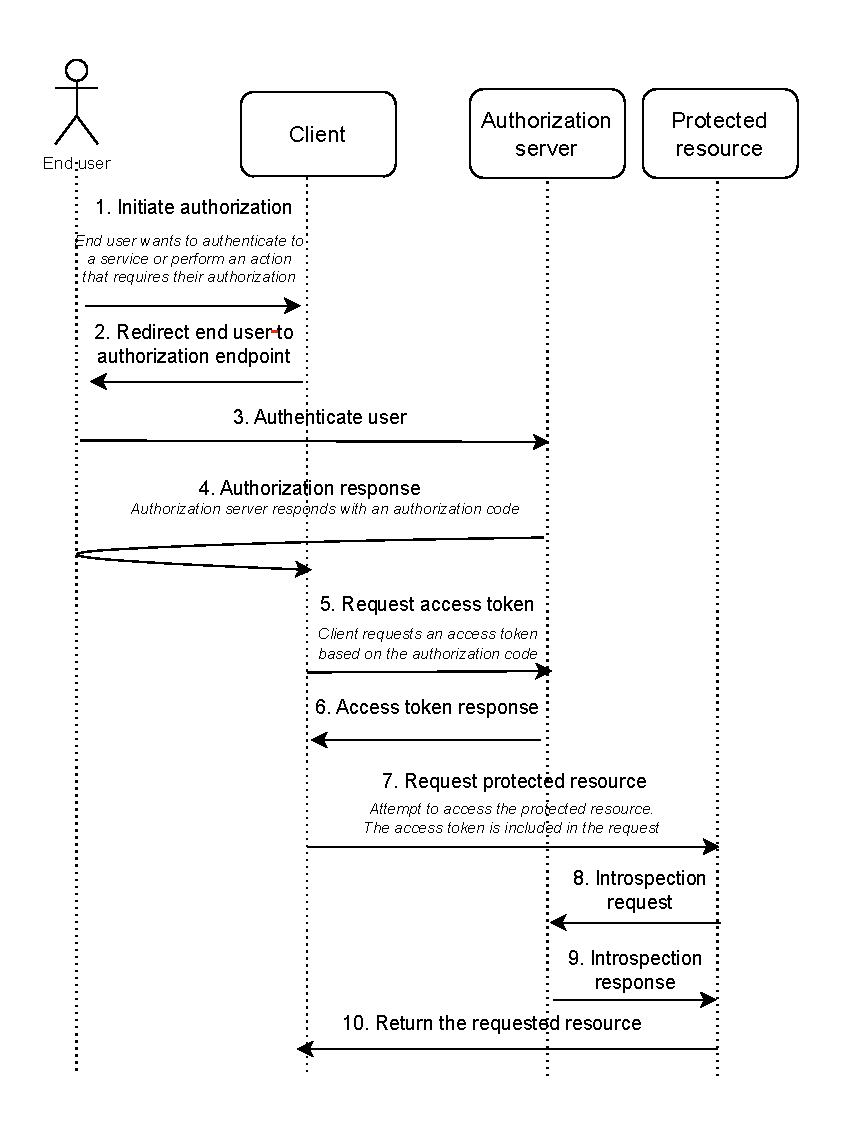
\includegraphics[height=190mm]{assets/oauth_authorization_code_grant.drawio.pdf}
	\caption{Accessing a protected resource using OAuth 2.0 authorization code grant.}
	\label{oauth_code_flow}
\end{figure}

\subsubsection{Implicit grant}
\label{sec:background-oauth-implicit}
Access tokens can also be obtained using the implicit grant type, which simplifies the authorization flow of the authorization code grant by removing the issuing of authorization codes.
This shortens the number of round-trips required, improving the responsiveness of interactive applications.
The steps of the implicit grant are similar to the authorization code grant described in figure \ref{oauth_code_flow}, with the authorization server responding with an access token directly, instead of issuing an authorization code first.
The implicit grant type removes the use of refresh tokens, requiring end users to authenticate multiple times if a session takes longer than the access token is valid.
As the access token is included in the response URI, there is an increased chance for the token leaking.
The implicit grant does not provide a method for identifying clients, making it impossible for authorization servers to validate that the used token was requested to the client using it.

\clearpage

\section{Vulnerabilities in OAuth systems}
\label{sec:vulnerabilities}

The OAuth protocol does not strictly define how systems utilizing the protocol should be implemented, requiring developers to thoroughly consider the security of their implementation choices.
When inspecting the security of OAuth systems, the critical components are the client and the authorization server.
Poorly implemented OAuth systems are very common, with Philippaerts et al. (2022) finding some vulnerability in each inspected authorization server \citep{philippaerts_oauch_2022}.
Client implementations are not any more secure, with Yang et al. (2016) finding simple mistakes in a majority of inspected web applications \citep{yang_model-based_2016}.
As these vulnerabilities are obvious enough to be found with automated methods, an attacker is very likely to find them as well.


\subsection{Vulnerabilities in authorization servers}
\label{sec:vulnerabilities-server}
As the authorization server is a trusted entity in the OAuth authorization flows, it is essential that it is securely implemented.
In addition to following general best practices for server management, such as keeping systems up to date, developers should consider OAuth-specific vulnerabilities.
To avoid on-path attackers, TLS should be used for all communication with the authorization server.
To lower the chance of developer mistakes, clients should be forced to use TLS for all communication with the authorization server.

\subsubsection{HTTP 307 redirect}
In the redirection-based authentication flows of the OAuth specification, how the redirections are implemented can have a significant impact on the overall security of the system.
While the choice of HTTP status code used for redirection is seen as an implementation detail in the OAuth specification, the status code used should be chosen carefully.
In contrast with other types of redirects, if the 307 HTTP status code is used as redirection, the body of the original POST request can be redirected.
If the authorization server uses HTTP 307 to redirect users to the client after authenticating, the client could receive the credentials that were originally sent in the body of the HTTP request to the authorization server.
If an attacker tricks a victim to authenticate to the legitimate authorization server through a malicious client, the attacker could receive the credentials  \citep{fett_comprehensive_2016}.

The 307 redirect attack is similar to a traditional phishing attack, where a victim is tricked to sign in to a malicious website, giving the attacker their credentials \citep{dhamija_why_2006}.
The 307 redirect attack is more likely to succeed compared to a traditional phishing attack, as it can be much harder to distinguish from a legitimate authentication.
In the attack, the victim authenticates to the legitimate authorization server, making it difficult to distinguish from a normal authentication.
Additionally, tricking the victim to visit the malicious client could be achieved in one single click, without the victim visiting the malicious site at any point, instead directly being directed to the legitimate authorization server.
As such, the victim does not have to miss subtle details in the login form that are slightly off, or mistake the malicious domain for a legitimate one as in traditional phishing attacks.

To clarify that the request body should not be sent together with the redirection, the HTTP code 303 should be used, as it explicitly states that the body should not be included in the response \citep{fielding_http_2022}.
Using a correct HTTP code does not solve the issue of sending credentials together with the client callback, as the authorization server can choose what content to send regardless of the status code used.
While correctly dropping the request body will have to be implemented by the authorization server, by using a HTTP status code that explicitly states that the request body should be dropped, the likelihood for faulty implementations is lower, compared to the 307 code which explicitly states that the original request body should be included in the redirect.

\subsubsection{Insecure token handling}
Due to the central role of tokens in OAuth authorization flows, their secure handling is essential.
In the authorization code flow the relevant tokens are access tokens, refresh tokens and authorization codes.
To avoid leaked tokens being abused, each token should only be valid for a short amount of time.
To extend the lifetime of user sessions and their corresponding access tokens, refresh tokens should be used.

In the authorization code grant, authorization codes are used to request an access token from the authorization server.
In a correct authorization code flow, the code should only be used once, and it should be used quickly after it has been granted.
As such, to avoid replay attacks, the authorization server should only be valid for one request, and it should have a short expiry time \citep{yang_security_2013}.
Additionally, if an authorization code is used multiple times, the authorization server should invalidate all related codes and tokens.
As an authorization code should never be used more than once in a correct code flow, duplicate use implies that something has gone wrong in the client or that an attacker is attempting a replay attack.

Refresh tokens should be dealt with similarly to authorization codes, being single use and only valid for a set amount of time.
The expiration time for refresh tokens can be longer than that of authorization codes, and can vary based on the specific client.
While the OAuth specification is quite clear in requiring the rotation of refresh tokens, Philippaerts et al. (2022) found that 44\% of authorization servers accept old refresh tokens that have already been used
\citep{philippaerts_oauch_2022}.
The old refresh tokens should be stored, and all related tokens should be invalidated if an old refresh token is used.
Compared to storing one old authorization code to detect replay attacks, detecting old refresh tokens can require storing a significant amount of tokens.
The large number of stored refresh tokens can require large amounts of storage, and the comparison to old refresh tokens can cause significant storage load \citep{darwish_evaluation_2015}.
As such, developers should weigh the benefits of storing old refresh tokens with the costs when deciding how long old tokens should be stored for.

\subsubsection{Redirect URI attack}
As the generated authorization code and refresh and access tokens are sent to the redirection URI, the authorization server has to validate that the redirect URI is correct.
The OAuth specification states that clients should register each allowed redirection URI, and that the authorization server should check the complete URI.
In practice, the redirect URI validation can be implemented in a number of ways.
While the minimum check should be to compare the complete redirect URI against a stored value, many authorization servers only check the origin of the redirect URI, allowing an attacker to change the path of the redirect URI \citep{matyas_your_2018}.
For increased security, authorization servers can also generate client-specific redirect paths when a client registers.

In the authorization code grant, the client sends the received authorization code to the authorization server to receive an access token.
Clients typically define a separate redirect URI for each provider, such as \textit{/oauth/callback/google} and \textit{/oauth/callback/amazon}.
If an attacker is able to tamper with the path of the redirection URI, with methods such as malicious images or iframes, the client could be tricked to send the code to the wrong provider \citep{matyas_your_2018}.
If the client application has an XSS vulnerability at a certain path, an attacker could set that vulnerable path as the redirect URI.
While OAuth tokens are generally secure against XSS as long as they are stored as HttpOnly cookies, if an attacker is able to execute code in the redirect flow they will be able to read the code or token that has been generated, as they are sent as query parameters to the client before being stored as a cookie.
This allows attackers to impersonate the victim, or to access protected resources belonging to the victim.

%\subsubsection{Clickjacking}
%Malicious iframes

%X-FRAME-OPTIONS DENY
\subsection{Vulnerabilities in OAuth clients}
When implementing OAuth-based authentication systems, a developer can choose to rely on external authorization servers, greatly simplifying the authentication logic they need to implement on their own.
When relying on external authorization servers, a developer is limited to studying the available providers and choosing ones that are suitable and secure.
This in turn allows developers to focus on implementing a secure client.
The most common client vulnerabilities are related to poor CSRF protections due to misuse of the \textit{state} parameter, poor tracking of user intent and incorrect token storage in the client.

\subsubsection{Invalid state handling}
\label{sec:vulnerabilities-state}
When used correctly, the state parameter provides protection against CSRF attacks \citep{almgren_more_2015}, with the OAuth 2.0 specification stating that the state parameters should be used for all authorization requests.
However, a 2016 study by Yang et al. found that 61\% of studied applications did not use the state parameter, while 55\% of applications that use state mishandled it in some way \citep{yang_model-based_2016}.
A study carried out by Almgren et al. (2015) was less pessimistic, but still found that 25\% of the Alexa Top 10 000 websites did not implement standard CSRF protections, such as correctly utilizing state \citep{almgren_more_2015}.

The OAuth authorization flows utilize redirects to provide access tokens and authorization codes to clients.
If the state parameter is not used by the OAuth client, clients have no way to verify how an authorization flow was initiated.
As such, if the state parameter is missing, many types of CSRF attacks become easier to execute for attackers.
The simplest form of CSRF attack that can be performed on clients that do not use the state value is the login CSRF attack.
In the login CSRF attack, a victim is tricked to authenticate to a legitimate site using the legitimate authorization server, but signing in the victim as the attacker.
This can lead to the victim performing operations as the attacker, and if the victim stores any information while they are logged in, such as payment information, the attacker will gain access to them.

Missing state validation can also be used to attack the federation process of an OAuth system that is used to sign in users \citep{chow_security_2014}.
The attack targets the account creation process, causing the victim's account on a relying site to bind to an account at the provider that is controlled by the attacker.
While the attack is similar to the login CSRF attack, it provides more persistent access to attackers, and has an increased probability of leaking the victim's personal information, as such information is typically provided when creating an account.

While state is used by many clients, it is not very useful if it is not implemented correctly.
Similar attacks can often be performed on clients mishandling the state parameter as on those that do not consider the parameter at all.
The state parameter should be random and difficult to guess, should ideally be single-use and should under no circumstances be shared between sessions or users.
Yang et al. (2016) identified a number of common mistakes in state validation \citep{yang_model-based_2016}:
\begin{itemize}
    \item \textbf{Lack of state validation} \\ 
    The state parameter is used but its value is never actually validated by the client
    \item \textbf{Lenient state validation} \\
    Some clients only validate the state parameter if it is provided. However, they do accept requests that are missing the state parameter.
    \item \textbf{State not bound to user} \\
    The client assumes that all state parameters that it has generated are valid but does not check which user the state parameter belongs to.
    This allows an attacker to perform a CSRF attack by substituting the victim's state with their own.
    \item \textbf{State not single use} \\
    If the state parameter is not single use, an attacker can use a previous parameter in a replay attack.
    The parameter could be obtained by eavesdropping or some other form of leaking.
    The risk for leaking the state parameter is especially high if TLS is not used. Some common characteristics of state reuse are keeping the same state value until the user tries to log in again, keeping the same state value as long as the user uses the same browser, or using a constant state value across all sessions and users.
\end{itemize}

%\subsubsection{Session integrity attack}


%\subsubsection{Poorly configured client authorization}


\subsubsection{IdP mix-up attack}
\label{sec:vulnerabilities-idp}

If the OAuth client fails to keep track of the authorization server that the user has chosen, an IdP mix-up attack could be performed by a network attacker \citep{fett_comprehensive_2016}.
In the IdP mix-up attack, a victim's authorization code or access token is sent to an authorization server controlled by an attacker.
To perform the attack, the OAuth client must allow multiple different authorization servers, and one of the allowed servers must be malicious.
In practice, this could occur if one authorization was compromised by attackers, providing them further access.
An attacker must also be able to modify requests sent to the OAuth client, which could be accomplished by an active network attacker.

The IdP mix-up attack in an authorization code flow is described in figure \ref{idp_mix_up}.
The request initiating authorization (request 1) is modified by an attacker, changing the chosen authorization server from the honest authorization server to a malicious server controlled by the attacker.
The client stores the choice of authorization server locally, and redirects the user agent to the malicious authorization server (requests 2 and 3).
The malicious server redirects the user agent to the honest authorization server, making it very difficult for the victim to notice anything out of the ordinary (request 4).
The end user authenticates normally to the honest authorization server, and the authorization server sends a response containing an authorization code to the OAuth callback route of the client (request 5).
As the client believes that the malicious authorization server should be used, it sends the authorization code to the malicious authorization server when it attempts to request an access token (request 6).
The malicious authorization server now has the victim's authorization code, and can request an access token (requests 7 and 8).
Having gained access to the access token, the attacker can now impersonate the victim or gain access to protected resources belonging to the victim \citep{tonetta_security_2017}.


\begin{figure}[b]
	\centering
    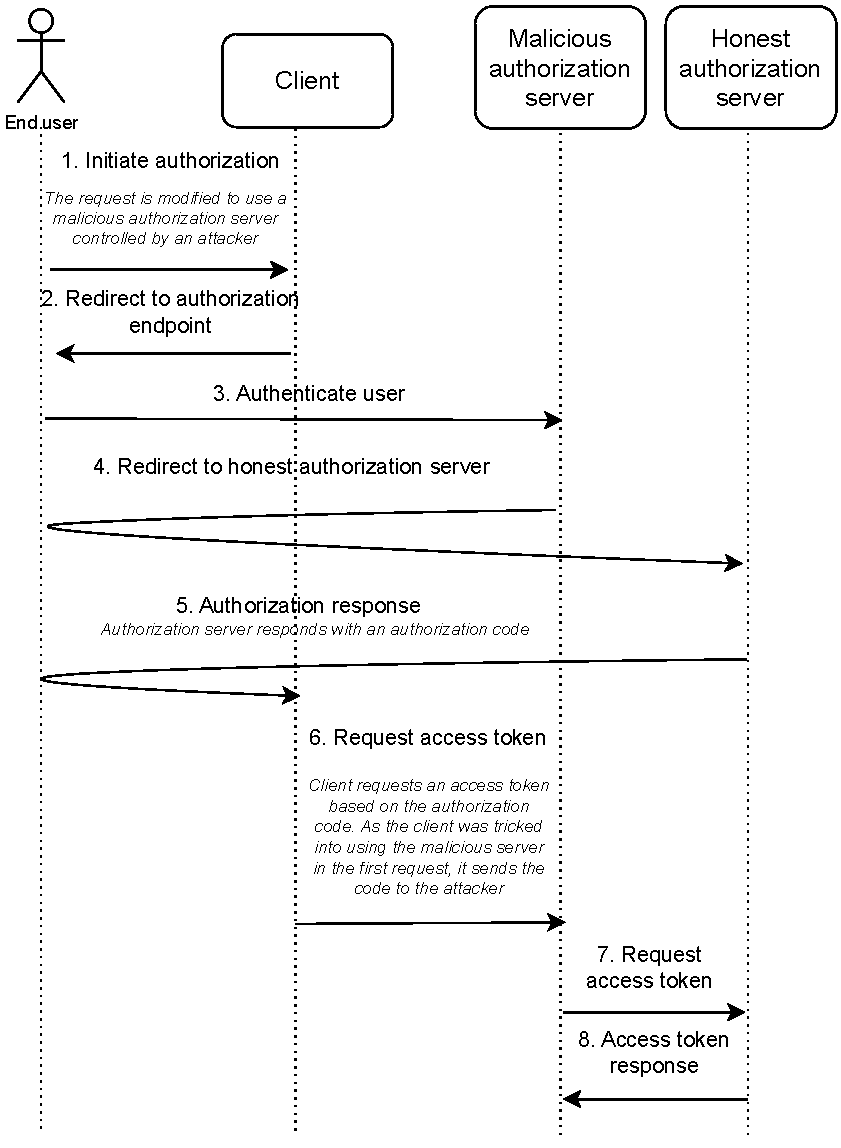
\includegraphics[height=185mm]{assets/idp_mix_up.drawio.pdf}
	\caption{IdP mix-up attack in an authorization code flow}
	\label{idp_mix_up}
\end{figure}

\subsubsection{Vulnerabilities in token storage}
When storing data in web clients, the user will be able to access the data, no matter how much a developer attempts to secure it.
Client-side storage such as cookies or local storage are also vulnerable to XSS attacks.
As such, if the goal is to maximize security, public clients should completely avoid persistent local token storage.

Even if persistent local storage is avoided, sensitive codes and tokens will have to be temporarily stored in JavaScript. 
Developers should consider how this temporary storage is implemented.
One possible hardening option is using JavaScript closures.
When using closures, the variables inside the closure can only be accessed by code inside the definition area of the closure, significantly reducing the chance that a XSS attack would succeed in gaining access to client secrets \citep{taly_automated_2011}.
Browsers also allow running code in web workers, which act as a separate thread.
In addition to allowing concurrent programming, web workers allow executing JavaScript code in an isolated sandbox.
Similarly to closures, this greatly reduces the risk of credentials leaking in case of an XSS attack, as the malicious code would have to be executed in the web worker containing the secret to be able to access it \citep{chinprutthiwong_security_2020}.

While persistent token storage has security issues, the added benefits provided by users being able to stay signed in across multiple sessions and browser restarts can outweigh the costs.
When persisting tokens, developers are limited to using the web storage API and storing session data in cookies.
Data stored using the web storage API and as cookies are limited to a specific domain, making it impossible for malicious sites to directly access the sensitive data.
Both methods are however vulnerable to XSS attacks, as they can be accessed using JavaScript.
When using cookies, XSS attacks can be mitigated by setting the \textit{HttpOnly} flag.
When the flag is set, the cookie can no longer be accessed by arbitrary JavaScript, with the cookie being included in requests to a specific domain.
The web storage API does not provide any protections similar to \textit{HttpOnly} cookies, and as such it should be avoided when storing any sensitive information.
As the cookie value is included in every request, this leaves additional room for potential CSRF attacks, making other types of CSRF protections, such as correctly utilizing the \textit{state} parameter even more critical.

\clearpage

\section{Implementing an OAuth client}
\label{sec:implementation}
This chapter describes a practical implementation for an OAuth 2.0 client using an authorization server provided by a third party.
The central design choices are described in addition to their effect on the security of the system.
The OAuth client consists of a minimal frontend application that interacts with an API backend which handles all communication with the authorization server.
The backend supports using multiple authorization servers simultaneously, with the example implementing authorization using Google and Microsoft accounts.
The focus of the chapter lies on the authorization code flow, as the process of retrieving an access token is the most critical part of an OAuth system.
It should also be possible to implement the authorization code flow in a similar way as in the example for a wide variety of different applications.
The chapter briefly describes token introspection and token refreshing, but as their implementation will vary greatly between different applications, they are not described in detail.
The complete source code for the client can be found on GitHub \citep{noauthor_backjonasoauth-client_nodate}.
 

\subsection{Application structure}

When implementing a modern web application, developers are left with a number of choices.
As described in section \ref{sec:background-structure}, the utilization of JavaScript allows developers to implement complete applications that are fully contained on the end user's machine.
When implementing an OAuth client, it is possible to contain all logic on the client machine.
This does however negatively affect the overall security of the system.
Single-page applications (SPAs), where all logic is contained in the browser, are considered public OAuth clients, as a user can access and study every part of the system.
In such clients, the authorization code flow can only be partially implemented, as it relies on the client proving its identity using a client secret.
As the client is completely stored in the user's machine, a malicious user can simply analyze the application and retrieve the secret value.
As the benefits provided by the authorization code flow are not fully realized in public clients, they often utilize the implicit grant instead, which is inherently less secure than the authorization code flow.

Due to these limitations of pure SPAs, the example implementation splits the OAuth client into a frontend and a separate API backend.
The user interacts with the frontend which in turn interacts with the API.
The API is responsible for all communication with the authorization server, allowing the client to securely store client secrets.
The separate API also makes it possible to more securely store access tokens and other secrets belonging to the end user.
These storage options are described in detail in sections \ref{sec:implementation-storage} - \ref{sec:pkce}.

\subsubsection{Obtaining an access token}
\label{sec:implementation:access-token}

The OAuth client implements the authorization code grant to authenticate users.
As the client is separated into two parts, some additional steps are required compared to a minimal authorization code grant.
The network traffic of the authorization flow is shown in figure \ref{client_auth_requests}.
Each step in the authorization flow is detailed below, with code snippets describing how they are implemented.

\begin{figure}[b]
	\centering
    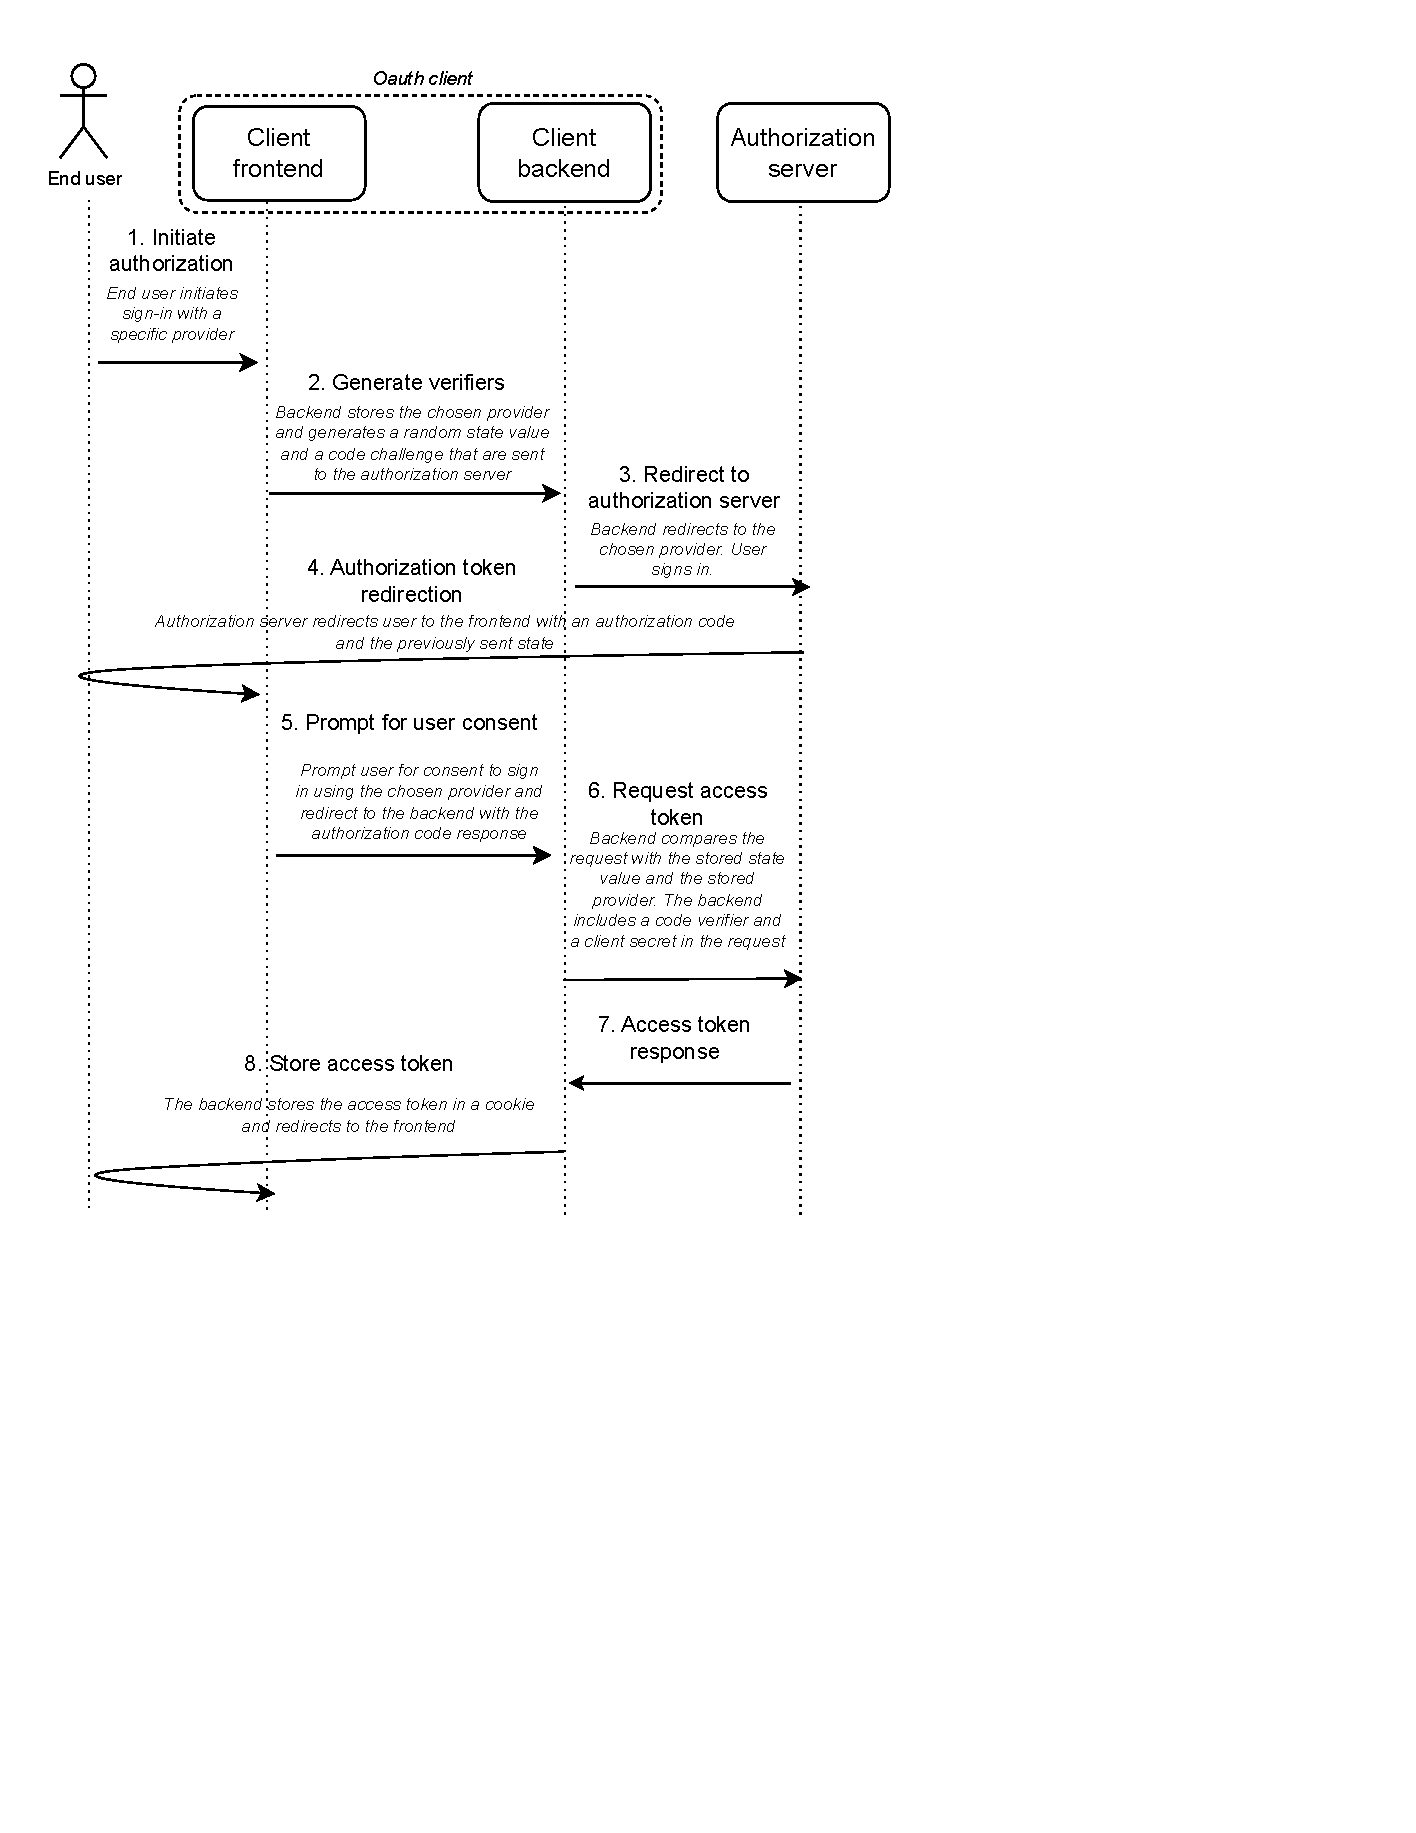
\includegraphics[height=185mm]{assets/client_request_flow.drawio.pdf}
	\caption{Network traffic of the OAuth clients authentication flow}
	\label{client_auth_requests}
\end{figure}

\clearpage
\begin{enumerate}
    \item \textbf{Initiate authorization} \\
    The user begins the sign-in process by clicking on a button to sign in with a specific provider.
\begin{lstlisting}[style=ES6, caption={Login button}]
const LoginButton = ({ provider }: { provider: string }) => {
  return (
    <button
      onClick={() =>
        (window.location.href = `${API_URL}/oauth/login/${provider}`)
      }
    >
      Login with {provider}
    </button>
  )
}
\end{lstlisting}
%\end{enumerate}

%\begin{enumerate}
%  \setcounter{enumi}{1}
    \item \textbf{Generate verifiers} \\
    The user is redirected to the client backend to a route belonging to the chosen provider.
    The backend server generates two random 32 byte strings, with one string used as a state value and the other string used as a code verifier.
    A code challenge is created based on the code verifier to be used by PKCE, described in more detail in section \ref{sec:pkce}.
    The backend stores the code verifier, the state value as well as the chosen provider as cookies in the user's browser. \\
    The code challenge is generated with the following function:
    \begin{lstlisting}[style=ES6, caption={Code challenge generation}]
export const generateCodeChallenge = (codeVerifier: string) => {
  return base64url(crypto.createHash('sha256').update(codeVerifier).digest())
}
\end{lstlisting}
    \item \textbf{Redirect to authorization server} \\
    The user is redirected to the chosen authorization server.
    The state and code challenge generated in the previous step are included as query parameters, in addition to a \textit{redirect URI}, to which the authorization server will redirect the user after successfully authenticating.
    A client id provided by the authorization server is also included, as well as the \textit{access\_type} which indicates whether a refresh token should be included. \\
    The URL to the authorization server is constructed with the following function:
    
\begin{lstlisting}[style=ES6, caption={Constructing the authorization server URL}]
export const getAuthServer = async (
  state: string,
  codeChallenge: string,
  provider: string
) => {
  const endpoint = await getEndpoint('authorization_endpoint', provider)
  const oauthCredentials = config.providers[provider]
  if (endpoint === undefined || oauthCredentials === undefined) {
    return undefined
  }

  // Refresh token should be requested as part of the scope  
  // for Microsoft, while it is requested from other
  // providers with access_type='offline'
  const scope = provider === 'microsoft' ? 'offline_access openid' : 'openid'

  return (
    endpoint +
    '?response_type=code' +
    `&client_id=${oauthCredentials.clientId}` +
    `&scope=${scope}` +
    `&redirect_uri=${config.redirectUri}/${provider}` +
    '&access_type=offline' +
    `&state=${state}` +
    `&code_challenge=${codeChallenge}` +
    '&code_challenge_method=S256'
  )
}
\end{lstlisting}

    The complete login route is implemented as follows, where \textit{oauthRouter} is an express router \citep{noauthor_express_nodate}:
\begin{lstlisting}[style=ES6, caption={Login route}]
oauthRouter.get('/login/:provider', async (req: Request, res: Response) => {
  const { provider } = req.params
  const state = randomBytes(32).toString('hex')
  const codeVerifier = base64url(randomBytes(32))
  const codeChallenge = generateCodeChallenge(codeVerifier)

  const authServer = await getAuthServer(state, codeChallenge, provider)
  if (authServer === undefined) {
    return res.sendStatus(500)
  }

  res.cookie('state', state, {
    httpOnly: true,
    secure: true,
    sameSite: 'lax',
    signed: true,
    maxAge: 60 * 1000,
  })

  res.cookie('code_verifier', codeVerifier, {
    httpOnly: true,
    secure: true,
    sameSite: 'lax',
    signed: true,
    maxAge: 60 * 1000,
  })

  res.cookie('provider', provider, {
    httpOnly: true,
    secure: true,
    sameSite: 'lax',
    signed: true,
  })

  res.redirect(authServer)
})
\end{lstlisting}

    \item \textbf{Authorization token redirection} \\
    After authenticating the user, the authorization server redirects the user to the client frontend, which was defined as a \textit{redirect URI}.
    The redirect includes an authorization code as well as the previously defined state parameter.
    \item \textbf{Prompt for user consent} \\
    The client asks the user to confirm that they wish to authenticate using the chosen provider.
    This step is not part of the authorization code grant flow, but is included as an additional guard against CSRF.
    The additional protection is needed, as a user could be tricked to initiate the authorization process by clicking a malicious link.
    As the user is redirected to this page by the \textit{redirect URI} parameter set in step 3, a user authenticating using a specific provider can only be redirected to one confirmation page, as long as the authorization server is not incorrectly configured.
    This protection is provided by the fact that authorization servers require setting all allowed redirect URIs, and as only one URI is needed for the flow, redirection can be limited to one allowed path per provider.
    After consenting to the authorization, the user is redirected to the backend, forwarding the authorization code and state parameter the authorization server sent. \\
    The consent page is implemented as the following React \citep{noauthor_react_nodate} component.

\begin{lstlisting}[style=ES6, caption={User consent page}]
import { useParams } from 'react-router-dom'

const API_URL = import.meta.env.API_URL

export const OAuthCallbackPage = () => {
  const { provider } = useParams()
  const { searchParams } = new URL(document.location.toString())
  return (
    <>
      <h1>Login confirmation</h1>
      {provider === undefined ? (
        <p>Authentication error</p>
      ) : (
        <>
          <p>Do you wish to continue authenticating using {provider}?</p>
          <button
            onClick={() =>
              (window.location.href = `${API_URL}/oauth/code/${provider}?${searchParams.toString()}`)
            }
          >
            Continue
          </button>
        </>
      )}
    </>
  )
}
\end{lstlisting}

    \item \textbf{Request access token} \\
    The backend fetches the state, code verifier and provider that were stored as cookies in step 2.
    The previously stored state and provider are compared with the values in the current request, and if either value does not match the authorization process is aborted.
    The following steps are taken to validate the request:
    \begin{lstlisting}[style=ES6, caption={Part of the backend code callback route that deals with validating the request}]
oauthRouter.get('/code/:provider', async (req: Request, res: Response) => {
  // Verify that a authorization code was provided
  // and that a code verifier has been stored in the client cookies
  const code = req.query?.code
  const codeVerifier = req.signedCookies?.code_verifier
  if (typeof code !== 'string' || typeof codeVerifier !== 'string') {
    return res.sendStatus(400)
  }

  // Verify that the state sent in the original authorization request matches
  // with the state provided in the callback
  const codeState = req.query?.state
  const cookieState = req.signedCookies['state'] as string | undefined
  if (
    typeof codeState !== 'string' ||
    typeof cookieState !== 'string' ||
    codeState === '' ||
    codeState !== cookieState
  ) {
    return res.sendStatus(403)
  }

  // Verify that the provider of the oauth callback matches with the
  // provider of the original login request
  const previousProvider = req.signedCookies?.provider
  const provider = req.params.provider
  if (
    typeof previousProvider !== 'string' ||
    typeof provider !== 'string' ||
    provider !== previousProvider
  ) {
    return res.sendStatus(403)
  }
  ...
})
\end{lstlisting}

    If all the validation steps pass, an access token is requested from the authorization server based on the authorization code.
    It includes the same client id as in the original authorization request, with an additional client secret.
    The original code verifier and redirect URI are also included. \\
    The access token is requested with the following function:
    \begin{lstlisting}[style=ES6, caption={Function used to request an access token and refresh token}]
export const getToken = async (
  code: string,
  codeVerifier: string,
  provider: string
): Promise<TokenResponse | undefined> => {
  const endpoint = await getEndpoint('token_endpoint', provider)
  const configCredentials = config.providers[provider]
  if (endpoint === undefined || configCredentials === undefined) {
    return undefined
  }

  const client_id = configCredentials.clientId
  const client_secret = configCredentials.clientSecret
  const redirect_uri = `${config.redirectUri}/${provider}`
  const grant_type = 'authorization_code'
  const code_verifier = codeVerifier

  try {
    const authResponse = await fetch(endpoint, {
      method: 'POST',
      body: new URLSearchParams({
        client_id,
        client_secret,
        redirect_uri,
        grant_type,
        code,
        code_verifier,
      }),
      headers: {
        'Content-Type': 'application/x-www-form-urlencoded',
      },
    })
    if (!authResponse.ok) {
      return undefined
    }
    return (await authResponse.json()) as TokenResponse
  } catch (error) {
    console.error(error)
    return undefined
  }
}
\end{lstlisting}
    \item \textbf{Access token response} \\
    The authorization server verifies the code verifier and checks that the redirect URI matches with the URI of the original code request.
    If the checks pass, the server responds with an access token, as well as an optional refresh token and id token, if they were requested in the code request.
    \item \textbf{Store access token} \\
    The backend stores the access token and optional refresh token as cookies and redirects the user to the landing page of the frontend.
    The token storage is described in greater detail in section \ref{sec:implementation-storage}.
    When the user makes a request to the backend in the future, the server will be able to identify the user based on this access token. \\
    The token storage and user redirection is handled as follows:
\begin{lstlisting}[style=ES6, caption={Part of the backend code callback route that deals with storing tokens and redirecting the user to the frontend}]
oauthRouter.get('/code/:provider', async (req: Request, res: Response) => {
  ...
  const token = await getToken(code, codeVerifier, provider)
  if (token !== undefined) {
    res.cookie('access_token', token.access_token, {
      httpOnly: true,
      secure: true,
      sameSite: 'strict',
      signed: true,
      maxAge: token.expires_in * 1000,
    })

    res.cookie('refresh_token', token.refresh_token, {
      httpOnly: true,
      secure: true,
      sameSite: 'strict',
      signed: true,
    })
  }

  res.redirect(config.frontendOrigin)
})
\end{lstlisting}
\end{enumerate}

\subsubsection{Inspecting existing access tokens}

OAuth access tokens are typically opaque, and as such a client can not extract any information from the token itself.
If an OAuth client wants to identify a user and confirm that an access token is valid, it must send an introspection request to the authorization server.
The token introspection flow is described in figure \ref{introspection_client_flow}.
The token introspection relies on an access token and a provider that were stored when obtaining an access token.
Many frontend libraries require explicitly including cookies to send them in any requests.
In our TypeScript example using the fetch() global function \citep{noauthor_fetch_2023}, cookies can be included with the \textit{credentials: 'include'} option.
The backend application must also set the Access-Control-Allow-Credentials header in the response to signal that cookies are used to identify requests.

Based on the type of token, the authorization server can return a differing amount of information, such as user emails and names.
The minimal information that it will return however is a unique \textit{sub} value, which is a unique identifier for the token subject.
When combining this sub value with the token provider, the OAuth client can identify a user, allowing the client application to serve personalized content.

\begin{figure}[b]
	\centering
    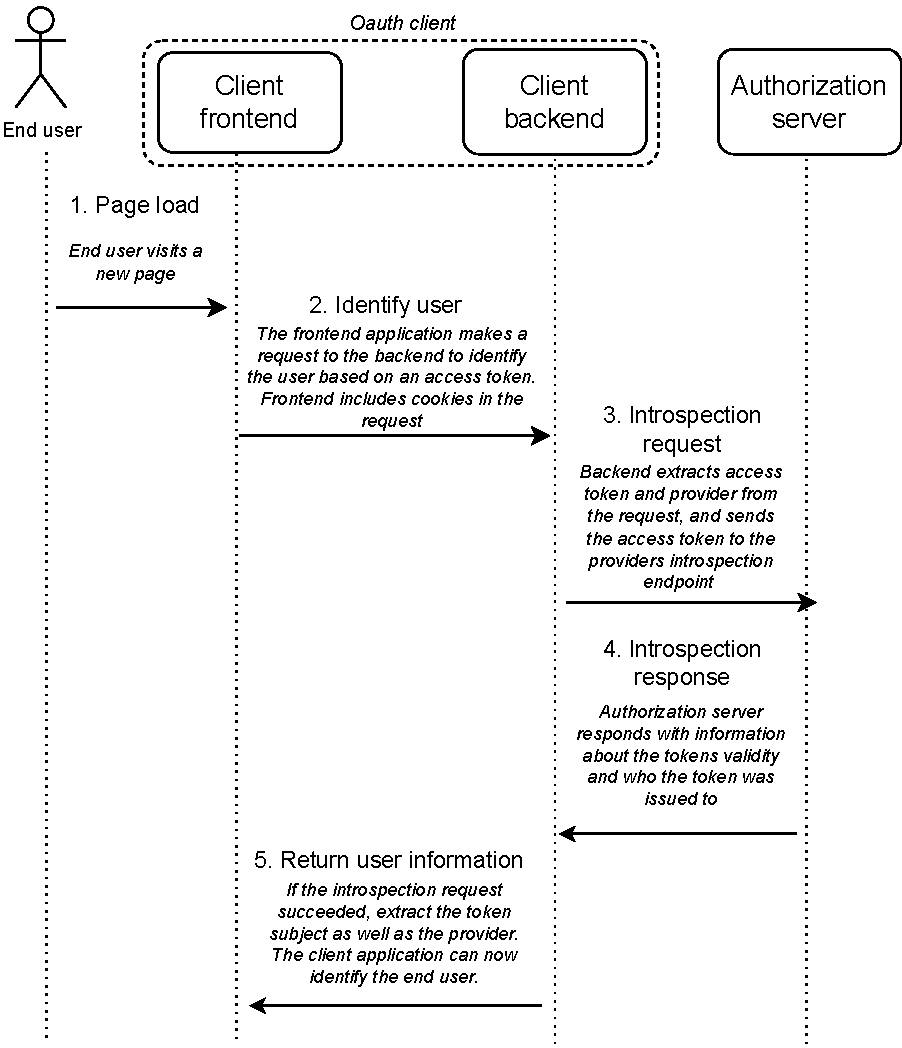
\includegraphics[height=165mm]{assets/introspection_client_flow.drawio.pdf}
	\caption{Network traffic of the access token introspection}
	\label{introspection_client_flow}
\end{figure}

\subsubsection{Refreshing access tokens}
Since access tokens are only valid for a specific time, it is useful to be able to refresh existing tokens, ideally without requiring user input.
To achieve this, OAuth clients can request refresh tokens, which can be used to request new access tokens.
While they do improve the user experience, refresh tokens weaken the security of the system, as their long expiry time increases the probability that they will be leaked.

In the client example, a refresh token is requested by setting the $access\_type$ to offline in the authorization code request (step 3 in figure \ref{client_auth_requests}).
The refresh token is then stored as a cookie in the end user's browser, similarly to the access token.
The refresh token can now be used when the client frontend interacts with the backend.
In the client example, the refresh token is used in combination with the token introspection request.
If a refresh token is set and the access token is not set, or if the introspection response fails (step 4 in figure \ref{introspection_client_flow}), the backend server will attempt to request a new access token based on the stored refresh token.
If the refresh succeeds, the client stores the updated access token and retries the earlier token introspection.
If the refresh fails, the refresh token and access token are removed.

\subsection{Token storage}
\label{sec:implementation-storage}
As described in section \ref{sec:background-storage}, a number of options exist for storing data in web browsers.
The most secure storage solution for an OAuth client would be to temporarily store tokens in JavaScript, with closures providing some additional security.
Such a solution would not however provide any persistence, and as such the end user would have to authenticate every time they start a new browser session.
To improve the user experience, the example client persists the access tokens, allowing users to stay logged in across multiple sessions.
When choosing to persist data developers have two practical options: the web storage API and cookies.
Due to its vulnerability to XSS attacks, the web storage API is not an optimal solution for storing sensitive information.
We instead opt for cookies to store any client-specific information when obtaining an access token, described in section \ref{sec:implementation:access-token}.

Many cookie flags that improve the storage security, described in section \ref{sec:background-storage}, are essential when storing sensitive data such as access tokens.
The cookies are marked as \textit{HttpOnly}, causing the cookies to be included in requests while keeping them completely inaccessible for the frontend application.
Instead, only the backend application can set and modify the cookies.
Any sensitive cookies should also be marked as \textit{Secure}, causing them to only be included in HTTPS requests.
This is a critical flag to include, as any network attacker could intercept sensitive cookies in transit if they are included in regular HTTP traffic.
Cookies should also have an appropriate \textit{SameSite} value.
The state, code verifier and provider should be stored with the \textit{Lax} SameSite policy, as they are accessed in a request that is initiated from the authorization server.
The access token and refresh token should instead be stored with the \textit{Strict} policy, as it does not need to be included in requests with any external origin.

To further limit the possibility of sensitive tokens leaking, tokens can be encrypted before storage.
Since all communication with the authorization server in an OAuth client with a separate frontend and backend flows through the backend server, the end user does not need access to the original, unencrypted access token, code verifier or OAuth provider.
If all the values stored in the client are encrypted, an attacker is unable to steal the original tokens.
The provided security benefit from this is however quite limited, as the client backend will accept and decrypt any token, without any way to verify if it was stolen or not.
Instead, the encrypted cookies have a greater impact on the authorization code flow, as modifying the temporarily stored state, code verifier or OAuth provider is more difficult.
An attacker is required to interact with the backend client themselves to obtain modified values that are encrypted with the correct key, allowing the client to limit what type of values are generated.
This also makes it easier to investigate malicious activity, since the attacker has to interact with the legitimate client to pull off any attack.
\subsection{Proof Key for Code Exchange}
\label{sec:pkce}
To protect against authorization code injection, the OAuth 2.0 Security Best Current Practice \citep{ietf-oauth-security-topics-27} recommends using Proof Key for Code Exchange (PKCE) to bind authorization codes to client instances \citep{rfc7636}.

PKCE relies on creating a code verifier in the initial authorization code request (step 2 in figure \ref{client_auth_requests}).
The code verifier should be a random string with between 43 and 128 characters.
This code verifier should be temporarily stored by the client.
In our example client, the value is stored as a cookie in the user's browser.
After generating the code verifier, the client generates a code challenge by hashing the code verifier.
The code challenge should be generated using the SHA256 algorithm \citep{dang_secure_2015} if possible.
The generated code challenge is sent to the authorization server together with the code request.
The used code challenge method, such as \textit{S256} if SHA256 is used, is also included in the request.

After receiving the authorization code, the OAuth client requests an access token from the authorization server (step 6 in figure \ref{client_auth_requests}).
The original code verifier is included in the access token request.
The authorization server computes a code challenge based on the verifier and the previously sent challenge method and compares it with the initial code challenge.
If the two code challenge values do not match, the authorization server interrupts the access token generation.




\subsection{Explicit user intention tracking}
To protect against CSRF attacks and IdP mix-up attacks, described in sections \ref{sec:vulnerabilities-state} and \ref{sec:vulnerabilities-idp}, additional controls should be used to keep track of user actions.
To alleviate these issues, the authorization code flow described in figure \ref{client_auth_requests} contains some additional checks that are not mandatory in the OAuth 2.0 authorization code flow described in figure \ref{oauth_code_flow}.
The chosen provider is tracked in each step, with separate routes for separate providers to limit the chance for a mix-up.
Additionally, the original chosen provider is stored as a cookie, allowing the client to validate that the actual used provider is the same as the provider chosen by the user.

Step 5 of figure \ref{client_auth_requests}  is also added as an extra guard against CSRF and IdP mix-up attacks.
The redirect via the frontend prompting for user consent is not required to request an access token, which could be handled completely in the backend.
It is however useful as a prompt for the user to confirm that they intend to sign in to the page, and that they chose to sign in with a specific provider.
If the step was missing, it is possible that an attacker could craft a CSRF request that signs in the user as the attacker, or that signs in the user using the wrong authorization server.

\clearpage

\section{Discussion}
This section discusses the findings of sections \ref{sec:vulnerabilities} and \ref{sec:implementation}, with discussion about the chosen implementation decisions and
other possible options as well as their benefits and drawbacks.
Observations from utilizing third-party authorization servers are also detailed, with a focus on how securely the servers are implemented, and how well they succeed in guiding developers to implement secure clients through their documentation.

\subsection{Client implementation options}
\label{sec:discussion-client-options}
When implementing an OAuth client, the security of two clients that both adhere to the OAuth 2.0 specification can be very different.
This is mainly due to the specification being quite lenient, with a significant portion of security-enhancing features defined as optional or recommended.
While this does have the benefit of allowing developers to create very simple OAuth clients that still adhere to the specification, the varying security can be misleading for end users that are likely to assume that all single sign-on systems are created equal.

\subsubsection{OAuth authorization flows}
A general design principle for our OAuth client is to do as much in the client backend as possible, as opposed to in the frontend.
While the frontend is a SPA and could thus do almost everything the backend does, every frontend operation has to consider the possibility that it could be tampered with by an attacker.
Keeping the frontend implementation as simple as possible also makes it easier to translate the logic to other languages or frameworks if required.
As described in section \ref{sec:implementation}, the separate client backend also allows keeping values secret from the end user, which is required to implement the authorization code flow, which should be wherever possible instead of the less secure implicit grant.

The authorization code flow requires the client to generate random values for the state and code verifier.
Generating random values is a very common problem with a number of viable solutions.
Our client uses the \textit{randomBytes} function from the \textit{crypto} module to generate these random values \citep{noauthor_crypto_nodate}.
The \textit{crypto} module has the benefit of being included in Node.Js by default, without requiring any additional third-party libraries.
The widespread use of the library also makes it more likely that any vulnerabilities are found and patched promptly.
The code challenge could also be sent in plain text, so that the code challenge and code verifier are the same string.
If possible, the code challenge should however be a hashed version of the code verifier.
The Node.Js \textit{crypto} module contains a function for generating the hash as well, \textit{createHash}, which is used in our client, using the SHA256 algorithm.
While authorization servers can choose to support other hashing algorithms, they are only required to support SHA256 and plain text code challenges \citep{rfc7636}.

Both the frontend and backend keep track of the used authorization server by using separate paths for separate providers.
The provider could be provided as a query parameter as well, with no impact on the security of the system.
It is however simpler to keep track of the provider in the path, as the authorization server redirect contains data as query parameters, which could potentially cause clashes with any additional data stored using the same parameters.
Other options are not available, such as sending the provider in the request body, as the provider has to be contained in the redirect URI sent to the authorization server.
By additionally storing the provider as a cookie, the backend server can confirm that the initial login request was using the provider that the user believes they are using when approving the login on the consent page.
This is necessary, as a user could be redirected to the confirmation page from any server with any parameters, legitimate or malicious, with no way to confirm where the redirect request originated.

The additional user consent screen is mainly intended as a defense mechanism against IdP mix-up attacks and CSRF attacks.
CSRF attacks generally rely on users clicking a link which has unintended side effects, such as causing the user to submit a form with the values as query parameters in the link.
While the client frontend does not have a form that can be submitted to initiate the login request, a link to the backend server with the correct URI would cause the user to be redirected to an authorization server.
As such, it has to be considered that the user could be redirected to the redirect URI defined in the authorization code request without ever knowingly agreeing to sign in.
Since the allowed redirect URIs have to be defined for each authorization server, if each provider has separate callback paths, a sign-in request from a legitimate authorization server can only redirect to their own callback path.
While it is still possible for an attacker to redirect a user to this confirmation page with malicious parameters, such as a code belonging to the attacker, the backend server should be able to catch these attacks by verifying the state and code verifier values.
The state and code verifier values created in the initial code request are only stored in the client's browser, and due to them being single-origin, the backend server must have set the cookies if they are able to read them.
If an attacker crafts a malicious link to request an access token based on the attacker's code, both the state and the code verifier checks will fail.
Additionally, since authorization servers should perform exact URI comparisons to verify that a redirect URI is allowed, an attacker is unable to embed any malicious content in the redirect URI itself.


\subsubsection{Persisting OAuth tokens}
While the improvements in user experience are clear when persisting access tokens using some client-side storage method, such as cookies in our example, long-time storage of tokens does make the system less secure.
While cookies marked as \textit{HttpOnly} are not accessible from applications running in the client browser, the end user is able to access them in the browser.
Any token that is stored runs the risk of falling into the wrong hands, which is why many critical applications, such as online banks, often do not allow users to stay logged in between multiple sessions.
Access tokens do mitigate this risk of leaking somewhat by being relatively short lived.

Refresh tokens are however not short lived, and as described in section \ref{sec:discussion-server-security}, authorization servers often allow refresh tokens to be used to request multiple access tokens, without having an expiration time for the refresh token.
As such, refresh tokens make the system less secure.
Furthermore, if refresh tokens are stored in the same place as access tokens, as is done in our OAuth client example, the benefits of having an expiration time on the access tokens are not realized, as it is equally likely for the refresh token and access token to be leaked, while the refresh token can be valid for a longer time increasing the chance that an attacker is able to exploit it.
This implies that refresh tokens should not be stored in cookies together with the access token, and in our client example this could be achieved by storing the refresh token in the client backend, which should limit the chance for these tokens to be leaked.
This immediately raises the requirements for developers and system administrators, as they are now responsible for implementing a secure storage method for these sensitive tokens.
This mitigates one of the main benefits of utilizing third party authorization servers, which is the lowered requirements for a developer wishing to implement a secure authorization system.

\subsection{Observations from utilizing third-party authorization servers}
\label{sec:observations}
A clear benefit of the OAuth 2.0 protocol is that it removes many complicated technical details from application developers, allowing them to rely on an established and trusted third party to implement the critical sign-in logic, leaving less room for mistakes.
For this benefit to materialize, the application developers should be able to find information on how clients can be implemented securely.
Additionally, as the third parties are trusted to implement the sign-in system securely, their authorization servers should be implemented correctly and securely.
This section describes the developer experience of using authorization servers provided by Google and Microsoft, with notes on how securely they are implemented.

\subsubsection{Quality of documentation}
\label{sec:observations-documentation}
Since developers using third party authorization servers might not be familiar with OAuth best practices, it is essential that documentation and examples show secure implementations.
As discussed in chapters \ref{sec:vulnerabilities} and \ref{sec:implementation}, a developer implementing an OAuth client has to make a number of decisions that have a significant impact on the security of the system.
Some of the areas where developers can make decisions that impact the system security are the choice of authorization flow, the use of state and PKCE and the use of refresh tokens.

As discussed in sections \ref{sec:background-oauth-code} and \ref{sec:background-oauth-implicit}, the authorization code flow should be preferred over the implicit grant flow whenever possible due to the greatly improved security.
Despite this, the Google documentation for client-side web applications state that the implicit grant flow is the only viable option for such clients \citep{noauthor_oauth_clientside}.
In contrast, Microsoft's version of the same documentation clearly states that the implicit grant flow is not a suitable authentication method today, and even states that existing applications using the implicit grant flow should migrate to using the authorization code flow\citep{owenrichards1_microsoft_2024}.

When utilizing the authorization code flow, using the state value is a simple way to protect against a number of attacks, as discussed in section \ref{sec:vulnerabilities-state}.
As such, it is a positive sign that both studied documentation sets recommend using the state value, and that the state value is included in example requests.
While the inclusion of the state value is positive, neither of the used documentation sets actually explain how or where the state value should be verified, leaving some room for improvement.

Similarly to the recommended authorization flow, Google and Microsoft seem to have a very different view on the importance of PKCE.
In the case of Google, PKCE is only described in their documentation for mobile and desktop applications \citep{noauthor_oauth_desktop}, while it is completely absent from their documentation for web servers \citep{noauthor_oauth_server}.
Even in the desktop documentation where PKCE is described, it is completely missing from the example requests, leaving it up to the developer to figure out how and where the \textit{code\_challenge} and \textit{code\_verifier} values should be included.
Microsoft's documentation on the other hand does describe PKCE, and the relevant parameters are included in the example requests.
Additionally, the Microsoft documentation recommends using PKCE for all application types and requires its use for single page applications that use the authorization code flow.

\subsubsection{Authorization server security}
\label{sec:discussion-server-security}
When choosing to use third-party authorization servers, developers rely on these third parties to securely implement the services.
Since the OAuth 2.0 specification is quite lax, an authorization server that complies with the specification can have a number of known vulnerabilities.
Details on how authorization servers are implemented are provided below, based on observations from utilizing Microsoft's and Google's authorization servers and the vulnerabilities listed in section \ref{sec:vulnerabilities-server}.

Supporting the use of state is essential when implementing secure OAuth clients.
As such, it is a positive note that the investigated authorization servers support the state parameter, and have implemented it correctly.
The state parameter is however optional, leaving room for developers to implement insecure clients.
While the state parameter is described as optional in the OAuth specification, authorization servers could encourage more secure practices by requiring users to provide a state value.
The state support does however leave room for improvement, as the servers do not support invalidating a code if a state validation fails.
While this code invalidation is not described in the OAuth specification, it does provide clear security benefits, as a failure to validate the state should only occur as a result of an error or some malicious activity.
As the authorization codes are single-use, this invalidation could be implemented by requesting and immediately invalidating an access token, but a more direct option would be useful.

Due to the distributed nature of the internet, sensitive traffic should never be sent without encryption.
Since OAuth deals with sign-in logic and user credentials, there is no reason why any of the communication should use plain HTTP.
Microsoft and Google seem to agree, since all their endpoints force clients to use HTTPS.
Microsoft also forces redirect URIs to use HTTPS, only allowing for localhost addresses to use plain HTTP.
Google does however allow using HTTP for non-local redirect URIs.
Since authorization codes and access tokens are sent to the redirect URI, any network attacker that is able to intercept the traffic would be able to read this sensitive data in plain-text.

Section \ref{sec:vulnerabilities-server} also discusses a number of other redirect-related vulnerabilities.
Both of the studied authorization servers correctly mitigate these vulnerabilities.
The HTTP 307 redirect vulnerability relies on authorization servers incorrectly redirecting the request body, potentially allowing clients to receive user credentials.
While both studied authorization servers use HTTP 302 instead of the 303 code recommended by Fett et al. (2016) \citep{fett_comprehensive_2016}, the body is correctly removed from the redirect response.
The redirect URI attack relies on authorization servers not performing exact redirect URI matching when comparing provided redirect URIs with the list of allowed URIs, such as only comparing the origin.
Both studied authorization servers do perform exact URI matching, and as such they are not vulnerable to the attack.

Insecure handling of tokens is another common source for vulnerabilities in authorization servers.
The studied authorization servers correctly implement authorization codes by only allowing them to be used once.
The validity times for the access tokens are also appropriate, with both the access tokens of both providers being valid for one hour.
Both providers do however implement refresh tokens in a less secure manner.
Ideally, refresh tokens should have a similar expiration time as access tokens, requiring clients to periodically renew the token to keep it valid.
Additionally, refresh tokens should be single use, with authorization servers returning the next refresh token in the access token refresh response.
Instead, both providers issue refresh tokens that do not expire.
Additionally, the same refresh token can be used to request multiple access tokens.
Due to these implementation choices, the risk for session hijacking is increased significantly due to old leaked refresh tokens still being valid.
On a positive note, the authorization servers do correctly invalidate refresh tokens when the related access token is invalidated.


\clearpage

\section{Conclusions}
\label{sec:conclusions}

This thesis studied common vulnerabilities of systems using OAuth 2.0 and presented methods that can be used to mitigate these issues.
The motivation behind the study was the widespread use of OAuth and the lax nature of the standard, allowing clients to be implemented with very different levels of security.
The goal of the thesis was to identify common vulnerabilities in OAuth systems and demonstrate how a client can be implemented securely.

A number of common vulnerabilities in OAuth clients and authorization servers were described, in addition to steps that can be taken to mitigate the vulnerabilities.
The studied vulnerabilities can be divided into two categories: vulnerabilities caused by incorrect authorization server or client implementations and vulnerabilities in OAuth systems that implement the bare minimum required by the specification.
Incorrect handling of the authorization code redirect is shown to be a common source for vulnerabilities, such as the redirect URI attack which is made possible by systems not implementing exact URI matching for the redirect URI and the HTTP 307 attack, which is enabled by authorization servers sending the original request body in the redirect response.
Vulnerabilities that are caused by systems implementing the bare minimum of the OAuth specification are most commonly related to not using the state parameter and authorization servers allowing unencrypted web traffic, either to their own authorization endpoint or when redirecting back to the client.

The practical client implementation of the study shows that implementing a secure OAuth client is simple, as long as a few crucial details are implemented correctly.
While the client is implemented using certain tools and frameworks, the implementation is simple enough that it should be possible to translate the logic to any language or framework of choice.
The client implementation also showed that developers can outsource a significant amount of complexity related to user authentication to third parties that provide authorization servers.
While the steps needed to implement a secure OAuth client are not complex, the lax nature of the OAuth specification makes it easy for developers to make insecure decisions if they are not familiar with the technologies used.

Many of the mitigations were shown to be simple and inexpensive to implement, with the OAuth specification describing a significant portion of the security enhancing techniques.
Techniques that are outside of the OAuth 2.0 specification, such as PKCE, are similarly shown to be simple and effective at preventing many vulnerabilities.
Due to how easy many of these mitigations are to implement, it is not obvious why they are not mandatory.
While a more secure specification will still have to be implemented correctly by developers, explicitly requiring more secure processes should help limit the number of vulnerabilities found in real world applications.



%% In a thesis, every section/chapter starts a new page, hence the \clearpage
\clearpage




\clearpage
%\bibliographystyle{unsrtnat}
%\bibliography{references}
\printbibliography

\end{document}
